\documentclass[sigplan,10pt,review,anonymous]{acmart}
\setcopyright{none}
%\usepackage{geometry}
%\usepackage[colorlinks]{hyperref}
\usepackage{ebproof}
%\usepackage{amsmath}
%\usepackage{amsthm}
%\usepackage{amssymb}
%\usepackage{libertine}
\usepackage{stmaryrd}
\usepackage{cmll}
\usepackage{tikz}
\usepackage{tikz-cd}
\usepackage{bbm}
\usetikzlibrary{calc}
\usepackage{minted}

%\newtheorem{definition}{Definition}
%\newtheorem{theorem}[definition]{Theorem}
\newtheorem{remark}{Remark}

\newcommand{\kw}[1]{\ensuremath{\mathsf{#1}}}
\newcommand{\refby}{\sqsubseteq}
\newcommand{\bdot}{\cdot}
\newcommand{\que}{{\circ}}
\newcommand{\ans}{{\bullet}}
\newcommand{\ifr}[1]{\mathrel{[{#1}]}}

\newcommand{\ISpec}{\mathbf{ISpec}}

\title{%
  Refinement Conventions:
  Composing Certified Compilers and Certified Abstraction Layers}

\begin{abstract} %{{{
Despite significant progress
in the development of certified software,
the lack of interoperability between
verification techniques is a major obstacle
to the construction of
large-scale, heterogeneous certified systems.
%
Compositional semantics
can help address this challenge
by providing a common mathematical framework
across certified components,
as proposed in recent work on
refinement-based game semantics.

To make this work,
one key challenge is to give
a formal account of
the relationship between
component interactions
at different levels of abstraction.
%
A partial answer is provided by CompCertO,
a certified C compiler
which uses a notion of \emph{simulation convention}
to relate source- and target-level interaction
between translation units.
%This facilitates compositionality
%for the correctness proofs of compiler passes,
%organizing them into a type structure
%reminiscent of double categories.

This paper introduces \emph{refinement conventions}
as an analogous construction
for refinement-based game semantics.
%
Refinement conventions generalize both
the simulation conventions of CompCertO
and the abstraction relations used in
certified abstraction layers.
%and give a proper strategy model
%for the language semantics of CompCertO.
%Refinement conventions can also be used
%to connect the concrete C and assembly language interfaces
%used in CompCertO
%with the more abstract signatures
%used in the strategy specification model
%of certified abstraction layers.
%This allows us to produce
We use them to
refine the bounded queue layer example of \citet{rbgs-cal}
into a concrete C implementation
whose correctness proof can be composed
with that of CompCertO.

%In practice,
%even compositional \emph{proof techniques}
%are usually formulated with respect to a
%non-compositional, operational semantics.

%We propose a general approach to
%specification, refinement and abstraction
%in the context of compositional semantics.
%As a case study,
%we apply this methodology to the certified compiler CompCert
%and its recent compositional extension CompCertO.
%This allows us to interface CompCertO with
%a particularly simple theory of certified abstraction layers.

%Recent work proposes to use game semantics for
%refinement-based verification
%of complex systems.
%However,
%mechanizing game semantics in a proof assistant presents many challenges.
%%in part due to the complexity of most game models,
%%and in part because the mathematics used in traditional descriptions of games
%%are ill-suited to a type-theoretic formalization.
%We show that the \emph{template games} of P.-A. Melli\`es,
%and a recently proposed \emph{algebraic} formulation of game semantics
%provide a viable approach.
%We mechanize a simple game model in the Coq proof assistant,
%enriched with a dually nondeterministic refinement ordering.
%The result allows us to extend existing verification frameworks
%in various directions.
%
%First,
%we use the model to provide a coarse-grained denotational semantics
%of CompCert program components,
%and use it to characterize and soundly implement
%the traditional C control operators \texttt{setjmp} and \texttt{longjmp}.
%We show that games makes it possible to
%model aspects of the execution environments of programs
%and demonstrate the verification of a system involving
%two separate processes communicating through a pipeline.
%
%Then,
%we develop a theory of certified abstraction layers
%within our new model.
%By decoupling certified abstraction layers
%from their low-level CompCert semantics,
%and by imposing a stronger typing discipline
%on layer interfaces and implementations,
%we address long-standing limitations on their compositionality.
%In particular,
%we verify a page allocator
%which can be used by an arbitrary number of
%independent clients.
\end{abstract}
%}}}

\begin{document}

\maketitle

\section{Introduction} %{{{

Guaranteeing the reliability of computer systems
is a long-standing challenge.
A modern computer system involves
layer upon layer of complex hardware and software components.
Each layer relies for its correct operation
on the layers below,
such that a defect in any of them
could prevent the overall system from
working as expected.

Certified software is one promising avenue of research
tackling this challenge.
However,
current methodologies do not address
the end-to-end certification of
large-scale, heterogeneous systems.

\subsection{Certified Software}

%A certified program comes with a formal specification,
%which describes with mathematical precision
%the expected behavior of program.
%In addition to the program itself,
%developers must then produce
%a formal proof of correctness,
%which can be easily and mechanically checked by a third party.

Certified software is accompanied by
a mechanized proof of correctness.
Under the most expansive approach,
the construction of a certified program
starts with a formal semantics 
for the language in use,
mechanized in a general-purpose proof assistant.
We must then formulate a mathematical specification
%delineating the desired behavior of the program
in terms this model,
and prove a correctness property
showing that the program indeed meets the specification.

Formal methods research
has developed an impressive array of
methods, tools and proof techniques
which can be used to carry out this task,
and researchers have constructed
certified versions of many key system components,
including
operating system kernels \cite{sel4,popl15},
compilers \cite{compcert},
and even processor designs \cite{...}.
Unfortunately,
building a system out of reliable components
is not enough to ensure
the reliability of the system as a whole.

\subsection{The Limits of a Piecemeal Approach}

Two components can interact in faulty ways
even when each one is perfectly reliable on its own term.
For example,
the assumptions made by one component
may not match the guarantees provided by another.
For example,
two perfectly functional logic gates which do not agree
on the voltages representing 0 and 1
will not interact in a predictable manner.

Beyond this,
we have to ensure that the components are assembled
in such a way that the they interact harmoniously
to realize a particular function---%
say, that compatible logic gates
connected in a certain way will indeed
implement a half-adder circuit.
To address this issue,
we must use the specifications of components as \emph{interfaces},
so that not only the components themselves,
but also their proofs of correctness
can be connected with each other
to build a larger overall certified system \cite{deepspec}.

%Building on these successes,
%there have been attempts to build larger certified systems
%out of these certified components,
%using their specifications as interfaces
%between their correctness proofs \cite{deepspec,etc}.

This is often challenging,
because different certified components
tend to use different semantic models and proof techniques.
As a result,
while researchers have been able to interface
particular components in this way \cite{something},
as of yet no general methodology has emerged
for composing independently certified components
into larger certified systems.

Fortunately,
the large body of research on compositional semantics
provides a staring point to develop such a methodology.
In particular,
game semantics provides a very general approach,
and recent work \cite{rbgs-cal,act21}
suggests that by extending this model
to account for specifications and refinement,
it may be possible to embed disparate certified components
into a common framework
where it would be possible to model their interactions
and compose correctness proofs
alongside their implementations.

\subsection{Connecting Levels of Abstraction}

As we build up more and more complex systems,
the techniques we use to model and reason about those systems
often have little in common with
the ones used to model and reason about the underlying components.
For example,
the mathematics of logical circuits---%
used to engineer microprocessors---%
have little in common with
the semantics of these processor's assembly languages,
which in turn work very differently from
the abstractions provided by the operating system or
the high-level languages used to develop application software.
As a result,
building large-scale certified systems
operating operate across layers of abstraction
will requires more than
modeling interactions across across their components.
We must also describe explicitly
the relationship between
different \emph{views} of the system
and of its components
at different levels of abstraction.

From an engineering perspective,
describing the relationship between
high-level abstractions and the
low-level implementation of
cross-component interactions is very common:
voltage vs. binary levels,
calling conventions for CPU architectures,
network protocols etc.
This phenomenon is also well-understood
in the context of imperative programming:
for example,
\emph{data refinement} has long been understood
in the context of Hoare logic and the refinement calculus
\cite{dataref}
and simulation relations are ubiquitous
in the context of operational semantics.
Yet in both of these examples,
abstraction only operates at the level of
\emph{internal states} of components.
By contrast,
there is little precedent
tackling this kind of abstraction
when it comes to the \emph{interactions} of
components with their environments,
of for
a systematic understanding of this phenomenon
is the context of denotational semantics.

\subsection{Contributions}

Certified software includes
a formal specification and
a proof of correctness.
A variety of techniques have been used
to construct certified
compilers, operating system kernels, \ldots

In its most general form,
certified software is built as follows.
The language used to describe the system being constructed
is given a mathematical semantics,
which is formalized in a general-purpose proof assistant.
A specification then describes
the properties expected of the system
in terms of its semantic interpretation.
A mechanized proof then establishes
with high confidence
that the system indeed satisfies these properties.

In principle,
the use of a general-purpose proof assistant
makes it possible to interface disparate certified components.
However in practice,
the maths we use for this makes it difficult.

\subsection{Compositional Verification}

In order to scale,
verification methods must be compositional:
it must be possible to break down the problem of verifying a large program
into subproblems of manageable size.
Small program components such as individual statements
can then be verified with reasonable effort, or even automatically.

In principle,
compositional semantics can help.
In practice,
people use compositional \emph{proof techniques},
shown to be sound directly wrt. operational semantics:
program logics,
logical relations on syntax,
certified abstraction layers.

Yet for large-scale heterogeneous systems,
compositional semantics is a must (b/c of generality ---
compositional proof techniques only operate
for a set language/framework).
Hence time is ripe to reexamine how
denotational semantics can fit within the practice of verification.

CompCertO gets some of the way there
but the model is designed to map onto
existing techniques and proofs in CompCert.
As a result,
it doesn't have the nice mathematical properties
which would enable
generality and large-scale reasoning.

\subsection{Compositional Semantics}

[Denotational semantics mostly been considered
as a theoretical endaevor whose goal is to
better understand programming languages and PL features
from a mathematical point of view:
what things does a language express,
how can its structures be characterized.
Gold standard = full completeness.]

Typical paper:
show a full abstraction result for language X or
a technique to support feature Y.
This leaves out
specifications, refinement, abstraction
which are the bread and butter of
large-scale system construction and verification.

To deploy compositional semantics in the context of verification,
we must shift somewhat from this emphasis:
\begin{itemize}
  \item The ability to represent specifications,
    which may or may not be definable as programs,
%    runs counter to insistence on definability,
%    although it could still be useful to identify
%    a subset of the domain which corresponds to
%    actual programs.
  \item The prominent role of \emph{abstraction} and \emph{refinement}
    in the context of verification
    means they have to be taken more seriously
\end{itemize}

Proposal: Idea of a hierarchy of models \cite{act21,lics20}.

Refinement-based game semantics.

\subsection{Contributions}

Two sides:
\begin{itemize}
  \item Theoretical contribution:
    show how to handle abstraction,
    as in different views of the same system
    at different levels of details,
    described using different concepts.
  \item Practical contribution:
    demonstrate connection between LICS'20 CAL and CompCertO,
    how to implement the bounded queue example.
\end{itemize}

\vspace{1em}
NB: with CAL abstraction only about internal states.
But CompCertO shows we also need to handle
the externally observable \emph{interactions}
between components.


%}}}

\section{Main Ideas} %{{{

[section describes how compositional semantics
can be used for verification:
use completely distributive lattices instead of domains;
they provide a language for specifications.
Formal adjunctions can be used to model abstraction
and construct a double category.]

Introduce the ring buffer example
to illustrate the concepts involved:
start with the code,
and the techniques /
psychological tools used by
software engineers
to reason about their code.
Then how can we give a formal account of that?

\subsection{Semantics} %{{{

In order to subject a given system to mathematical analysis,
we must establish a mathematical model of its operation.
A programming language semantics
does this in a systematic way
by assigning to each program $p \in P$
in a given language $P$
a description $\llbracket p \rrbracket \in D$
of its behavior within a domain $D$:
\[
    \llbracket {-} \rrbracket : P \rightarrow D
\]

There are many approaches
for constructing appropriate domains
and interpretation functions.
What distinguishes \emph{compositional} semantics
is that the interpretation function $\llbracket - \rrbracket$
can be defined alongside the syntactic structure of programs.
For example,
if two program phrases $p_1, p_2 \in P$
can be combined into $p_1 + p_2 \in P$,
the semantic domain will be equipped with an operation
$\oplus : D \times D \rightarrow D$
such that
\[
  \llbracket p_1 + p_2 \rrbracket =
  \llbracket p_1 \rrbracket \oplus
  \llbracket p_2 \rrbracket
  \,.
\]

When \emph{types} are involved,
the syntax and semantics
can be given in \emph{categorical} form.
The syntax is given as a category $\mathbf{P}$
where objects are types and typing contexts,
and where the morphisms $p : \Gamma \rightarrow A$
are program components which
are assigned type $A$ within a context $\Gamma$,
or more generally
which use resources in $\Gamma$ to provide an interface $A$.
The interpretation function
the becomes a functor
$\llbracket - \rrbracket : \mathbf{P} \rightarrow \mathbf{D}$
into a semantic category $\mathbf{D}$,
such that a program $p : \Gamma \rightarrow A \in \mathbf{P}$
is interpreted as
a morphism
$\llbracket p \rrbracket :
 \llbracket \Gamma \rrbracket \rightarrow
 \llbracket A \rrbracket
 \in \mathbf{D}$.

%}}}

\subsection{Specifications and Refinement} \label{sec:specs} %{{{

From the perspective of certified software engineering,
semantics allows us to formulate specifications and
correctness proofs
in the context of a well-behaved mathematical domain.
To make specifications and proofs compositional,
we can impose additional structure.

A desirable property of program behaviors
can be expressed as a predicate $\pi \in \mathcal{P}(D)$
of the semantic domain.
Moreover,
a set $\Pi \subseteq \mathcal{P}(D)$
of properties of interest
induces a \emph{refinement} ordering
${\sqsubseteq} \subseteq D \times D$
over the semantic domain.
A behavior $\sigma \in D$ is refined by $\tau \in D$
when %the following holds:
\[
  \sigma \sqsubseteq \tau \: :\Leftrightarrow \:
  \forall \pi \in \Pi \bdot
  \pi(\sigma) \Rightarrow \pi(\tau)
  \,.
\]
Conversely,
if the domain is equipped \emph{a priori}
with a partial order $\sqsubseteq$,
then its elements can themselves be regarded as properties:
\[
  \Pi \: := \:
    \{ \tau \mapsto \sigma \sqsubseteq \tau \mid
       \sigma \in D \}
\]

When $D$ is rich enough,
this means that specifications themselves
can be interpreted as elements of the domain,
and the correctness of a program $p \in P$
with respect to a specification $\sigma \in D$
can be expressed as
\[
  \sigma \sqsubseteq \llbracket p \rrbracket
  \,.
\]
Under this refinement-based approach,
specifications and correctness proofs
benefit from the compositionality of $\llbracket - \rrbracket$.
For example,
when $\sigma_1 \sqsubseteq \llbracket p_1 \rrbracket$
and $\sigma_2 \sqsubseteq \llbracket p_2 \rrbracket$,
we can deduce:
\begin{equation} \label{eqn:speccomp}
  \sigma_1 \oplus \sigma_2 \:\sqsubseteq\:
  \llbracket p_1 \rrbracket \oplus
  \llbracket p_2 \rrbracket \:\sqsubseteq\:
  \llbracket p_1 + p_2 \rrbracket
  \,,
\end{equation}
as long as $\oplus$ is monotonic
with respect to refinement.

\paragraph{String Diagrams}

For categorical semantics,
these structure generalize to
order-enriched categories.
Every homset $\mathbf{D}(A, B)$
is equipped with a refinement ordering,
and the composition operation
\[
  {\circ}_{A,B,C} :
    \mathbf{D}(B, C) \times \mathbf{D}(A, B) \rightarrow
    \mathbf{D}(A, C)
\]
is a monotonic function.
Order-enriched categories can be seen as
\emph{thin} 2-categories,
where for $f, g : A \rightarrow B \in \mathbf{D}$
there is a 2-cell
$\alpha : f \Rightarrow g : A \rightarrow B$
if and only if $f \sqsubseteq g$.
Hence,
refinement proofs can be formulated as
\emph{string diagrams}.

In such a diagram,
the objects of $\mathbf{D}$ are represented by regions of the plane.
A morphism $f : A \rightarrow B \in \mathbf{D}$
is represented by a vertical line
separating an $A$ region from a $B$ region,
and a refinement property
$f \circ g \circ h \sqsubseteq u \circ v$
is represented as a point
connecting the lines $f$, $g$, $h$ above the point
to the lines $u$, $v$ below:
\[
  \text{[figure here]}
\]
For example,
property (\ref{eqn:speccomp}) above
combines the properties
(a) $\sigma_1 \subseteq \llbracket p_1 \rrbracket$ and
(b) $\sigma_2 \subseteq \llbracket p_2 \rrbracket$ with
the compositionality property
(c) $\llbracket p_1 \rrbracket \circ \llbracket p_2 \rrbracket
     \sqsubseteq \llbracket p_1 + p_2 \rrbracket$
in the following way:
\[
  \text{[figure here]}
\]

String diagrams
provide a visual calculus for refinement proofs where
the associativity and monotonicity of composition
are made implicit.

%}}}

\subsection{Game Semantics} %{{{

A particular kind of compositional semantics
known as \emph{game semantics} uses
categories of games and strategies
as semantic domains.
The games used in this context are
two-player games
which model the interaction between
a program component (the proponent)
and its environment (the opponent).
Then the behavior of a program component
is described by a proponent \emph{strategy}
in the game associated with the component's type.
The games do not usually involve
a winning condition or notion of payoff.

In the context of heterogeneous certified systems,
this approach is interesting
because games provide a fairly general way to describe
the interfaces of certified components.
For the purposes of the work presented here,
we will use particularly simple games
induced by the following notion of signature.

\begin{definition}
An \emph{effect signature} is a set $E^\que$ of operations
together with a family of sets $\big( E^\ans \big)_{m \in E^\que}$
specifying an \emph{arity} for each operation.
We will write
\[
  E = \{ m : E^\ans_m \mid m \in E^\que \}
\]
\end{definition}

The associated game simply consists of
a question $m \in E^\que$ from the environment,
followed by an answer $n \in E^\ans_m$ from the system.
We will be more interested in the composite game $E \rightarrow F$,
which allows the \emph{system} to ask questions in $E$
before answering the environment's initial question in $F$.

At a high level of abstraction,
the interface provided by the C program shown in \autoref{fig:rb}
and used by the C program shown in \autoref{fig:bq}
can be described using the signature:
\[
  E_\kw{rb} := \{
    \kw{inc1} {:} \mathbb{N},
    \kw{inc2} {:} \mathbb{N},
    \kw{set}[i, v] {:} \mathbbm{1},
    \kw{get}[i] {:} V \mid
    i \in \mathbb{N}, v \in V \}
\]
Note that there are individual operations
$\kw{set}[i, v]$ and $\kw{get}[i]$
for every possible value of the arguments
$i \in \mathbb{N}$ and $v \in V$.
In such circumstances,
we will sometimes use the notation
\[
  E_\kw{rb} := \{
    \kw{inc1} : \mathbb{N}, \:
    \kw{inc2} : \mathbb{N}, \:
    \kw{set} : \mathbb{N} \times V \rightarrow \mathbbm{1}, \:
    \kw{get} : \mathbb{N} \rightarrow V \}
  \,.
\]
Using this convention,
the interface provided by the program in \autoref{fig:bq}
can be described as the following signature:
\[
  E_\kw{rb} := \{
    \kw{enq} : V \rightarrow \mathbbm{1},
    \kw{deq} : V \}
\]

\paragraph{Plays and Strategies}

The program $\kw{bq.c}$
\emph{uses} the interface $E_\kw{rb}$ to
\emph{provide} the interface $E_\kw{bq}$.
Hence, its behavior
can be described as a proponent strategy for the game
$E_\kw{rb} \rightarrow E_\kw{bq}$.
Given a particular value $\diamond \in V$,
a \emph{play} in this game may look like the sequence of moves:
\[
  \kw{enq}[\diamond] \cdot
  \underline{\kw{inc2}} \cdot
  7 \cdot
  \underline{\kw{set}}[7, \diamond] \cdot
  * \cdot
  \underline*
  \:,
\]
where we have underlined moves of the proponent
and $* \in \mathbbm{1}$ is the unit value.
Traditionally,
\emph{strategies} are then defined as
the set of plays a component can generate,
depending on the environment's behavior.
For example,
the strategy
$\sigma_\kw{bq} : E_\kw{rb} \rightarrow E_\kw{bq}$
associated with $\kw{bq.c}$ is
\begin{align*}
  \sigma_\kw{bq} =
  \{ 
   &\kw{deq} \cdot
    \underline{\kw{inc1}} \cdot
    i \cdot
    \underline{\kw{get}[i]} \cdot
    v \cdot
    \underline{v} \,, \\
   &\kw{enq}[v] \cdot
    \underline{\kw{inc2}} \cdot
    i \cdot
    \underline{\kw{set}[i, \diamond]} \cdot
    * \cdot
    \underline*
  \mid
    v \in V, i \in I
  \}
  \,.
\end{align*}
Strategies of this kind can be ordered by
the set inclusion relation $\subseteq$.

\paragraph{Composition}

Suppose the strategy
$\sigma_\kw{rot} : E_\kw{bq} \rightarrow E_\kw{rot}$
implements %the signature
$E_\kw{rot} = \{ \kw{rot} : V \}$
with the following behavior:
\[
  \sigma_\kw{rot} := \{
    \kw{rot} \cdot
    \underline{\kw{deq}} \cdot
    v \cdot
    \underline{\kw{enq}[v]} \cdot
    * \cdot
    \underline{v}
    \mid v \in V
  \}
\]
That is,
an incoming call to $\kw{rot}$
uses the interface $E_\kw{bq}$
to first dequeue a value $v$,
push it back at the end of the queue,
then returns $v$.

The composite strategy
$\sigma_\kw{rot} \circ \sigma_\kw{bq} :
 E_\kw{rb} \rightarrow E_\kw{rot}$
lets the two components interact,
by replacing the calls
$\underline{\kw{deq}} \cdot v$
and
$\underline{\kw{enq}[v]} \cdot *$
in the plays of $\sigma_\kw{rot}$
by corresponding plays of $\sigma_\kw{bq}$.
The internal interactions between the two components
are then hidden to obtain the strategy:
\begin{align*}
  \sigma_\kw{rot} &\circ \sigma_\kw{bq} = \\
  \{
   &\kw{rot} \cdot
    \underline{\kw{inc1}} \cdot i \cdot
    \underline{\kw{get}[i]} \cdot v \cdot
    \underline{\kw{inc2}} \cdot j \cdot
    \underline{\kw{set}[j,v]} \cdot * \cdot
    \underline{v}
  \mid {} \\
   &i \in \mathbb{N}, \:
    j \in \mathbb{N}, \:
    v \in V
  \}
\end{align*}

%}}}

\subsection{Interaction Specifications} %{{{

We have discussed in \S\ref{sec:specs}
the relationship between
properties, refinements and specifications.
One way to look at the construction of strategies
in game semantics
is to read plays as elementary properties
of the system being modeled.

Within a strategy,
a play essentially states:
``if the environment behaves in this way,
then the system should respond in that way''.
Program components are then characterized by
the set of such properties which they satisfy.
Under-constrained strategies can be refined by
more defined ones.
Over-constrained strategies---%
which contain plays
making incompatible demands of the system---%
cannot be implemented by concrete programs.

The union of $\sigma_1$ and $\sigma_2$
can only be refined by strategies which refine both:
\[
  \sigma_1 \cup \sigma_2 \subseteq \tau
  \quad\Leftrightarrow\quad
  \sigma_1 \subseteq \tau \:\wedge\:
  \sigma_2 \subseteq \tau
  \,.
\]
In other words,
unions correspond to \emph{angelic nondeterminism},
where the environment is free to rely on either behavior
because the system must be capable of delivering both.
However,
to establish a complete refinement calculus
we also need a form of \emph{demonic nondeterminism},
allowing us to formulate specifications such as
``the system may either return 0 or 1''.


unions of strategies 

 correspond t

The union of strategies can only be refined
by a strategy which 

Strategy \emph{specifications} can then be expressed as
under-constrained sets of plays.
A component which refines them must admit 


\subsection{Completely Distributive Lattices}

It is well-understood that
semi-lattices provide the algebraic foundation
of traditional nondeterminism.
Completely distributive lattices
provide a similar foundation for
dual nondeterminism with arbitrary angelic and demonic choices.

\begin{definition}
A \emph{complete lattice}
is a partially ordered set $\langle L, {\le} \rangle$
with all joins and meets.
This means in particular that $L$
has a least element $\bot = \bigvee \varnothing = \bigwedge L$
and a greatest element $\top = \bigwedge \varnothing = \bigvee L$.
A \emph{completely distributive} lattice
is a complete lattice which satisfies
the (equivalent) distributivity properties:
\begin{gather} \label{eqn:compdist}
  \bigvee_{i \in I} \bigwedge_{j \in J_i} x_{ij} =
  \bigwedge_{f \in \prod_i J_i} \bigvee_{i \in I} x_{i,f_i}
  \\
  \bigwedge_{i \in I} \bigvee_{j \in J_i} x_{ij} =
  \bigvee_{f \in \prod_i J_i} \bigwedge_{i \in I} x_{i,f_i}
\end{gather}
\end{definition}

These properties admit an intuitive game-theoretic interpretation.
Suppose the elements of $L$
are \emph{payoffs} in a zero-sum, two-player games
where the proponent and opponent
take turns making moves.
The proponent seeks to minimize the payoff.
If they can choose among the payoffs $(x_i)_{i \in I}$,
the outcome will be $\bigwedge_i x_i$.
Conversely,
if the opponent can choose among $(y_j)_{j \in J}$,
the outcome will be $\bigvee_j y_j$.
Hence the expression
$\bigwedge_i \bigvee_j x_{ij}$
denotes the result of a game where
the proponent first makes a choice $i \in I$,
the opponent then chooses $j \in J_i$,
producing the outcome $x_{ij}$.

We can reverse the order of these moves
by having the opponent play first
and choose a strategy $f \in \prod_i J_i$.
The proponent then selects $i \in I$,
leading to the outcome is $x_{i,f_i}$.
At first glance,
this game is very different:
the proponent has access to much more information
and can make a decision based on the opponent's choice of strategy.
However,
the expressions $\bigwedge_i \bigvee_j x_{ij}$
and $\bigvee_f \bigwedge_i x_{i,f_i}$
are only concerned with the case where both players adopt
an optimal strategy.
In this particular scenario,
the opponent choices were in effect already known,
hence the proponent gains no advantage.

%}}}

\subsection{CompCertO}

\subsection{Certified Abstraction Layers}

\subsubsection{Abstraction Layers}

Remark on the role of layers in actual engineering.
But compositionality is not the only thing going on.
For developers,
there is a very important psychological advantage:
by introducing a new layer we also introduce
a new language,
new concepts,
new reasoning principles.

in introducing a new layer,

\subsubsection{Specifications and Refinement}
\subsubsection{Compositional Semantics}
\subsubsection{Game Semantics}
\subsubsection{Dual Nondeterminism}

\begin{figure}
\begin{minted}{C}
 /* Encapsulated state */
 static int c1, c2;
 static V buf[N];
 
 /* Accessors */
 int inc1() { int i = c1++; c1 %= N; return i; }
 int inc2() { int i = c2++; c2 %= N; return i; }
 V get(int i) { return buf[i]; }
 void set(int i, V val) { buf[i] = val; }
\end{minted}
\caption{The state of a ring buffer,
  made of two counters and a fixed-size array,
  is encapsulated behind a simple interface.}
\label{fig:rb}
\end{figure}

\begin{figure}
\begin{minted}{C}
 /* Underlay signature */
 extern int inc1(void);
 extern int inc2(void);
 extern V get(int i);
 extern void set(int i, V val);

 /* Layer implementation */
 void enq(V val) { set(inc2(), val); }
 V deq() { return get(inc1()); }
\end{minted}
\caption{This component relies on the ring buffer primitives
  provided in Fig.~\ref{fig:rb} to implement a bounded-size queue.}
\label{fig:bq}
\end{figure}
%}}}

\begin{figure*} % fig:cal {{{
  \begin{minipage}{.9\textwidth}
    \begin{align*}
      %
      % Overlay
      %
      & \fbox{$L_\kw{bq}$} &
        S_\kw{bq} &:= V^* \\
      \kw{enq} &: V \rightarrow \mathbbm{1} &
        L_\kw{bq}.\kw{enq}(v)@\vec{q} &:= \{ * @ \vec{q} v \mid |\vec{q}| < N \} \\
      \kw{deq} &: \mathbbm{1} \rightarrow V &
        L_\kw{bq}.\kw{deq}(*)@\vec{q} &:= \{ v @ \vec{p} \: \mid \vec{q} = v \vec{p} \}
      \\[1em]
      %
      % Implementation
      %
      & \fbox{$M_\kw{bq}$} &
        R &\subseteq S_\kw{bq} \times S_\kw{rb} \\
      M_\kw{bq}.\kw{enq}(v) &:= i \leftarrow \kw{inc}_2 ; \: \kw{set}(i, v) &
        \vec{q} \mathrel{R} (f, c_1, c_2) &\Leftrightarrow
        \: (c_1 \le c_2 < N \wedge
            \vec{q} = f_{c_1} \cdots f_{c_2-1}) \vee {}
      \\
      M_\kw{bq}.\kw{deq}(*) &:= i \leftarrow \kw{inc}_1 ; \: \kw{get}(i) &
        & \qquad \! (c_2 \le c_1 < N \wedge
            \vec{q} = f_{c_1} \cdots f_{N-1} f_0 \cdots f_{c_2 - 1})
      \\[1em]
      %
      % Underlay
      %
      & \fbox{$L_\kw{rb}$} &
        S_\kw{rb} &:= V^N \times \mathbb{N} \times \mathbb{N}
      \\
      \kw{set} &: \mathbb{N} \times V \rightarrow \mathbbm{1} &
        L_\kw{rb}.\kw{set}(i, v)@(f, c_1, c_2) &:=
        \{ *@(f', c_1, c_2) \mid i < N \wedge f' = f[i := v] \}
      \\
      \kw{get} &: \mathbb{N} \rightarrow V &
        L_\kw{rb}.\kw{get}(i)@(f, c_1, c_2) &:=
        \{ f_i@(f, c_1, c_2) \mid i < N \}
      \\
      \kw{inc}_1 &: \mathbbm{1} \rightarrow \mathbb{N} &
        L_\kw{rb}.\kw{inc}_1@(f, c_1, c_2) &:=
        \{ c_1@(f, c_1', c_2) \mid
           c_1' = (c_1 + 1) \mathop{\mathrm{mod}} N \}
      \\
      \kw{inc}_2 &: \mathbbm{1} \rightarrow \mathbb{N} &
        L_\kw{rb}.\kw{inc}_2@(f, c_1, c_2) &:=
        \{ c_2@(f, c_1, c_2') \mid
           c_2' = (c_2 + 1) \mathop{\mathrm{mod}} N \}
    \end{align*}
  \end{minipage}
  \caption{
    A certified abstraction layer
    $L_\kw{rb} \vdash_R M_\kw{bq} : L_\kw{bq}$
    implementing a bounded queue of size $N$
    using a ring buffer.
    The left-hand side of the figure shows
    the signatures of the overlay and underlay interfaces,
    and the code associated with the layer.
    The right-hand side shows primitive specifications
    and the simulation relation used by the correctness proof.
    Reproduced from \citet{rbgs-cal}.}
  \label{fig:cal}
\end{figure*}
%}}}

\section*{Interaction Specification Algebras} %{{{

[I am giving up on this section.
It is not really required for the main points the paper makes
and it is challenging to articulate everything in that context.
I will just review interaction specifications
in the main ideas section
and write another paper on algebraic game semantics.]

\begin{color}{gray}
[Briefly describe the LICS'20 model
for the sake of being self-contained.
Ideally, provide a characterization
as a free monad of some kind,
but this seems to be challenging.]

The work presented in this paper
builds on the \emph{interaction specification} model
of certified abstraction layers \cite{lics20}.
In this section,
we give a proper categorical characterization
of this model as a free monad,
which provides reasoning principles for
interaction specifications
independent of the particular construction
used to defined them.

\subsection{Overview} %{{{

The \emph{free monad} construction \cite{freemon}
has important applications in programming language semantics.
In particular,
it provides a bridge between
the traditional monadic approach
to modeling computational side-effect \cite{moggi}
and the constructions and techniques of universal algebra.
While monads in general do not compose easily,
algebraic theories enjoy a rich and uniform
composition framework.
By characterizing monads in terms of
the algebraic theories that induce them,
we can take advantage of this framework.

Recent work also connects the algebraic approach
to game semantics.
For simple games,
the traditional strategy construction
can be characterized as an initial algebra
in the category of
directed-complete partial orders and
strict Scott-continuous functions \cite{act21}.
Likewise,
the \emph{interaction specification} model
used as a starting point for our work
is inspired by both
game semantics and
algebraic effects.
However,
while \citet{lics20} presents its interaction specification monad
as a variation on the traditional free monad construction,
it does not provide a formal account of this assessment.

In this section,
we give a presentation of
the interaction specification monad
as a free monad.
This establishes the algebraic basis for the model,
and a more principled approach to inductive proofs.

%}}}

\subsection{Free Monad}

\subsection{Completely Distributive Lattices} %{{{

It is well-understood that
semi-lattices provide the algebraic foundation
of traditional nondeterminism.
Completely distributive lattices
provide a similar foundation for
dual nondeterminism with arbitrary angelic and demonic choices.

\begin{definition}
A \emph{complete lattice}
is a partially ordered set $\langle L, {\le} \rangle$
with all joins and meets.
This means in particular that $L$
has a least element $\bot = \bigvee \varnothing = \bigwedge L$
and a greatest element $\top = \bigwedge \varnothing = \bigvee L$.
A \emph{completely distributive} lattice
is a complete lattice which satisfies
the (equivalent) distributivity properties:
\begin{gather} \label{eqn:compdist}
  \bigvee_{i \in I} \bigwedge_{j \in J_i} x_{ij} =
  \bigwedge_{f \in \prod_i J_i} \bigvee_{i \in I} x_{i,f_i}
  \\
  \bigwedge_{i \in I} \bigvee_{j \in J_i} x_{ij} =
  \bigvee_{f \in \prod_i J_i} \bigwedge_{i \in I} x_{i,f_i}
\end{gather}
\end{definition}

These properties admit an intuitive game-theoretic interpretation.
Suppose the elements of $L$
are \emph{payoffs} in a zero-sum, two-player games
where the proponent and opponent
take turns making moves.
The proponent seeks to minimize the payoff.
If they can choose among the payoffs $(x_i)_{i \in I}$,
the outcome will be $\bigwedge_i x_i$.
Conversely,
if the opponent can choose among $(y_j)_{j \in J}$,
the outcome will be $\bigvee_j y_j$.
Hence the expression
$\bigwedge_i \bigvee_j x_{ij}$
denotes the result of a game where
the proponent first makes a choice $i \in I$,
the opponent then chooses $j \in J_i$,
producing the outcome $x_{ij}$.

We can reverse the order of these moves
by having the opponent play first
and choose a strategy $f \in \prod_i J_i$.
The proponent then selects $i \in I$,
leading to the outcome is $x_{i,f_i}$.
At first glance,
this game is very different:
the proponent has access to much more information
and can make a decision based on the opponent's choice of strategy.
However,
the expressions $\bigwedge_i \bigvee_j x_{ij}$
and $\bigvee_f \bigwedge_i x_{i,f_i}$
are only concerned with the case where both players adopt
an optimal strategy.
In this particular scenario,
the opponent choices were in effect already known,
hence the proponent gains no advantage.

%}}}

\subsection{Multimorphisms of Complete Lattices}

In $\mathbf{Set}$,
where we can reason about fully defined,
terminating programs,
notion of algebra so signature is easy:
\[
    \alpha : \sum_m \prod_n A \rightarrow A
\]
In other words,
for each operation $(m : N) \in E$
we give a function $\alpha^m : A^N \rightarrow A$,
which gives the interpretation of a computation
invoking the effect $m$
with the possible continuations $(k_n)_{n \in N} \in A^N$.

\subsection{Tensor Products}

Tensor products in $\mathbf{CDLat}$
are difficult to pin down.
In particular,
there is no such thing as a \emph{bicomplete} homomorphism
of non-trivial complete lattices,
since the required properties:
\begin{align*}
  f \left( \bigsqcap_{i \in I} x_i, y \right) &=
    \bigsqcap_{i \in I} f(x_i, y) &
  f \left( \bigsqcup_{i \in I} x_i, y \right) &=
    \bigsqcup_{i \in I} f(x_i, y) \\
  f \left( x, \bigsqcap_{i \in I} y_i \right) &=
    \bigsqcap_{i \in I} f(x, y_i) &
  f \left( x, \bigsqcup_{i \in I} y_i \right) &=
    \bigsqcup_{i \in I} f(x, y_i)
\end{align*}
are contradictory---%
consider for example $f(\bot, \top)$.

Explain how demonic choices must distribute
over environment choice of argument,
vs. angelic choices just move as in $\prod A_i \rightarrow A$.

\subsection{Interaction Algebras}

\subsection{Interaction Specifications}

\end{color}

%}}}

\section{Semantics in CompCert} %{{{

[This is mostly from my thesis,
I need to rewrite it to be more compact and specialized.]

[Explain how we can embed CompCertO semantics
for the purpose of CAL:
categorical/layered composition only,
don't care about footprints until the end,
angelic interpretation.]

In its strongest form,
the compiler correctness theorem proved in CompCert
is expressed as a forward simulation of labeled transition systems.
This simulation is then used to derive
a trace containment property.

Although CompCertO provides an updated notion of forward simulation,
in the compositional setting
it is challenging to
formulate a theorem analogous to trace containment.
To do so,
we must incorporate component interactions
into event traces.
Traces then become typed in the same way our transition systems are.
Because they include internal notions of state and interaction
which differ between the source and target languages,
the corresponding traces are no longer directly comparable,
and we must bring simulation conventions into the picture.

This is challenging because
simulation conventions involve
\emph{dual} nondeterminism:
both the system and the environment contribute choices
which determine how C-level behavior is realized at the assembly level.
Because of this,
neither trace inclusion (angelic nondeterminism)
nor trace containment (demonic nondeterminism)
are sufficient to express the relationship
between these behaviors.

\emph{Refinement-based game semantics} \cite{koenig20}
offers a solution,
in the form of a relatively simple game model
with full support for both angelic and demonic choices.
We have mechanized this model in the Coq proof assistant.
In this section,
we demonstrate how the compositional semantics used in CompCertO
can be interpreted in this setting.

%% preamble {{{
%
%The semantics of CompCert languages
%are given in terms of a simple notion of process behavior.
%By \emph{process}, I mean a self-contained computation
%which can be characterized by
%the sequence of system calls it performs.
%%Several steps are involved to go
%%from a source program to an executing process;
%%these steps are modeled by CompCert
%%with varying degrees of sophistication and accuracy.
%For a C program to be executed as a process,
%its translation units must be compiled to object files,
%then linked together
%into an executable binary
%loaded by the system.
%
%\begin{figure} % fig:process {{{
%  \centering
%    \begin{tikzpicture}[scale=1.25]
%        \tt
%        \node (Ms) at (1.5, 1) {whole-program.s};
%        \node (M1c) at (0, 3) {M1.c};
%        \node (M2c) at (1, 3) {M2.c};
%        \node (etc) at (2, 3) {\ldots};
%        \node (Mnc) at (3, 3) {M$n$.c};
%        \node (M1s) at (0, 2) {M1.s};
%        \node (M2s) at (1, 2) {M2.s};
%        \node (ets) at (2, 2) {\ldots};
%        \node (Mns) at (3, 2) {M$n$.s};
%        \draw (M1c) edge[->] (M1s);
%        \draw (M2c) edge[->] (M2s);
%        \draw (Mnc) edge[->] (Mns);
%        \draw (M1s) edge[->] (Ms);
%        \draw (M2s) edge[->] (Ms);
%        \draw (Mns) edge[->] (Ms);
%        \rm
%        \node at (-1.3, 2.5) {Compilation};
%        \node at (-1.3, 1.5) {Linking};
%
%        %\node (Mb) at (1.5, 0) {Running process};
%        %\node at (-1.3, 0.5) {Loading};
%        %\draw (Ms) edge[->] (Mb);
%
%        %\tt
%        %\node (Mc) at (1.5, 4) {whole-program.c};
%        %\draw (M1c) edge[->,dotted] (Mc);
%        %\draw (M2c) edge[->,dotted] (Mc);
%        %\draw (Mnc) edge[->,dotted] (Mc);
%    \end{tikzpicture}
%    \caption{CompCert's approximation of the C toolchain}
%    \label{fig:process}
%\end{figure}
%%}}}
%
%%Finally, the system loads the executable into memory
%%where initialization code sets up the process
%%and invokes the program's \texttt{main} function.
%%Since CompCert is a compiler from C to assembly,
%%but does not include an assembler or linker,
%The model used for verifying CompCert accounts for this
%in the way depicted in Figure~\ref{fig:process}.
%%The lowest-level objects considered
%%are CompCert \kw{Asm} programs.
%Linking is approximated by
%merging programs, seen as sets of global definitions.
%The execution
%of a program composed of the translation units
%$\texttt{M1.c} \ldots \texttt{M$n$.c}$
%which compile to
%$\texttt{M1.s} \ldots \texttt{M$n$.s}$
%is modeled as:
%\[
%    L_\kw{tgt} :=
%    \kw{Asm}[\texttt{M1.s} +
%             \cdots +
%             \texttt{M$n$.s}] \,.
%\]
%Here,
%$+$ denotes CompCert's linking operator and
%$\kw{Asm}$ maps an assembly program to its semantics.
%Note that the loading process is encoded
%as part of the definition of $\kw{Asm}$,
%which constructs a global environment
%laying out the program's code and static data
%into the runtime address space,
%and models the conventional invocation of \texttt{main}.
%To formulate compiler correctness,
%we must also specify the behavior of the source program.
%To this end,
%CompCert defines a linking operator
%and semantics
%for the language $\kw{Clight}$,%
%\footnote{
%  Although CompCert features a frontend for a richer version
%  of the C language,
%  the simplified intermediate dialect \kw{Clight}
%  is usually used as the source language
%  when using CompCert to build certified artifacts.
%  %In particular it is the target language of the
%  %\texttt{clightgen} utility which
%  %produces Coq code for a C program's AST,
%  %which the user can then prove to be correct
%  %either manually or with tools such as the VST program logic
%  %\citep{vst}.
%}
%allowing the desired behavior to be specified as:
%\[
%    L_\kw{src} :=
%    \kw{Clight}[\texttt{M1.c} + \cdots + \texttt{M$n$.c}] \,.
%\]
%Given an appropriate notion of refinement,
%the correctness of CompCert
%can then be stated as:
%\[
%  L_\kw{src} \refby L_\kw{tgt}
%  \,.
%\]
%
%%}}}

\subsection{Transition systems} %{{{

The semantics of CompCert languages are
given as labelled transition systems (LTS),
which characterize a program's behavior in terms of
sequences of observable events,
taken from a fixed set $\mathbb{E}$.

Schematically, a CompCert LTS
is a tuple
$L = \langle S, I, {\rightarrow}, F \rangle$
consisting of
a set of states $S$,
a subset $I \subseteq S$ of initial states,
a labelled transition relation
${\rightarrow} \subseteq S \times \mathbb{E}^* \times S$,
and a set
$F \subseteq S \times \kw{int}$
of final states associated with exit statuses.
The relation~$s \stackrel{t}{\rightarrow} s'$
indicates that the state $s$ may transition to the state $s'$
with the externally observable interaction $t \in \mathbb{E}^*$.

The execution of $L$ starts by selecting an initial state $s_0$,
then uses the transition relation to repeatedly update the state,
until a final state is reached:
\[
  I \ni s_0
  \xrightarrow{t_1} s_1
  \xrightarrow{\epsilon} s_2
  \xrightarrow{t_2} s_3
  \mathrel{F} r
\]
Roughly speaking,
the externally observable behavior of the program
consists of the sequence of events generated by transitions
($t_1 t_2$ in the execution above),
together with the exit status of the process
($r$ in the execution above).
See the next section for a more detailed account.

Note that nondeterministic choices
are potentially involved at every step of the execution:
the selection of an initial state from the set $I$,
the selection of a possible transition $\{ (t, s') \mid s \xrightarrow{t} s' \}$,
and the selection of an outcome $\{ r \mid s \mathrel{F} r \}$.
If there is a possible transition out of a final state $s$,
there will also be a choice of whether the execution should terminate
or continue.

The angelic, demonic, or mixed nature of these choices
is key to understanding CompCert's
notions of \emph{determinacy} and \emph{receptiveness}
of transition systems,
and the distinction and correspondence between
CompCert's notions of \emph{forward} and \emph{backward} simulations.

%}}}

\subsection{Behaviors} %{{{

I outlined above the execution of a labelled transition system
in terms of terminating traces.
The model used in CompCert is more general,
and defines four kinds of behaviors:
\begin{itemize}
\item As before, an execution reaching a final state is said to
    \emph{terminate}.
    For example,
    the following execution generates
    the event trace $t_1 t_2 \cdots t_{n-1}$
    and terminates with status $r$:
    \[
        I \ni s_1 \stackrel{t_1}{\rightarrow}
          s_2 \stackrel{t_2}{\rightarrow}
          \cdots \stackrel{t_{n-1}}{\rightarrow}
          s_n \mathrel{F} r
    \]
    We will write this behavior as
    \[
      t_1 t_2 \cdots t_{n-1} \Downarrow r
      \,.
    \]
\item An execution reaching
    an infinite sequence of $\epsilon$ transitions
    is said to \emph{silently diverge}.
    The following execution diverges after
    generating the trace $t_1 t_2 \cdots t_{n-1}$:
    \[
        I \ni s_1 \stackrel{t_1}{\rightarrow}
          s_2 \stackrel{t_2}{\rightarrow}
          \cdots \stackrel{t_{n-1}}{\rightarrow}
          s_n \stackrel{\epsilon}{\rightarrow}
          s_{n+1} \stackrel{\epsilon}{\rightarrow}
          \cdots
    \]
    We will write the corresponding behavior as
    \[
      t_1 t_2 \cdots t_{n-1} \Uparrow
      \,.
    \]
\item By contrast,
    infinite executions which keep interacting
    are said to exhibit \emph{reactive} behavior.
    The following execution
    is reactive if and only if
    $\forall i \bdot \exists j \ge i \bdot t_j \ne \epsilon$:
    \[
        I \ni s_1 \stackrel{t_1}{\rightarrow}
          s_2 \stackrel{t_2}{\rightarrow}
          s_3 \stackrel{t_3}{\rightarrow}
          \cdots
    \]
    Then the behavior of the transition system
    is represented by the infinite sequence
    \[
      t_1 t_2 t_3 \cdots
      \,.
    \]
\item Finally, an execution which reaches a stuck state
    is said to \emph{go wrong}. It will have the shape
    \[
        I \ni s_1 \stackrel{t_1}{\rightarrow}
          s_2 \stackrel{t_2}{\rightarrow}
          \cdots \stackrel{t_{n-1}}{\rightarrow}
          s_n \,,
    \]
    with no $t, s'$ such that
    $s_n \stackrel{t}{\rightarrow} s'$
    and no $r$ such that $s_n \mathrel{F} r$.
    This partially defined behavior is written
    \[
      t_1 t_2 \cdots t_{n-1} \lightning
      \,.
    \]
    It is refined by any behavior
    admitting $t_1 t_2 \cdots t_{n-1}$ as a prefix.
\end{itemize}
A transition system with no initial state ($I = \varnothing$)
immediately goes wrong.
In this case,
the transition system will admit the single undefined behavior
$\epsilon \lightning$.

Summing up,
the traces used by CompCert to define
the possible behaviors of transition systems
are taken from the following language:
\[
  b \in \mathbb{B} =
    \mathbb{E}^*
      \{ {\Downarrow} r, {\Uparrow}, {\lightning} \mid r \in \kw{int} \}
      \cup
    \mathbb{E}^\omega
  \,.
\]
We will write
${\refby_\lightning} \subseteq \mathbb{B} \times \mathbb{B}$
for CompCert's notion of \emph{behavior improvement},
which allows behaviors which go wrong to
be refined by more defined ones.
It can be defined as
\[
  {\refby_\lightning} := \{ (b, b) \mid b \in \mathbb{B} \}
    \cup \{ (t \lightning, t b) \mid
            t \in \mathbb{E}^*, b \in \mathbb{B} \}
  \,.
\]
Then the overall external behavior
of a transition system $L$
is characterized
as a set $\kw{Beh}(L) \subseteq \mathbb{B}$
of possible individual behaviors.
In the remainder of this section we will describe
the techniques used in CompCert to define and establish
corresponding notions of refinement.

%I will often simply write $b \in L$
%to mean that the transition system $L$
%admits the behavior $b$,
%overlooking the distinction between $L$
%and the set of behaviors it admits.

%}}}

\subsection{Events} %{{{

The events used in the traces above are taken from the following set:
\begin{align*}
  e \in \mathbb{E} ::=
    \kw{syscall}[u, \vec{v}]/v & \mid
    \kw{vload}[i, o]/v \\ \mid
    \kw{vstore}[i, o, v] & \mid
    \kw{annot}[u, \vec{v}]
\end{align*}
They correspond to system calls ($\kw{syscall}$),
volatile loads and stores ($\kw{vload}$, $\kw{vstore}$),
and annotations ($\kw{annot}$).
The data involved
are strings ($u \in \kw{string}$),
global identifiers ($i \in \kw{ident}$),
pointer offsets ($o \in \mathbb{Z}$) and
event values ($v \in \kw{eval}$, $\vec{v} \in \kw{eval}^*$).
Crucially,
these data are invariant between the source and target programs,
so that the corresponding traces can be compared directly.
For the purposes of this discussion,
the exact nature and use of these events
are not important,
but they correspond to the external interactions
which need to be preserved between the execution
of the source and target program.

Events involve both an output component,
chosen by the program and
written here to the left of the oblique bar ($/$),
and a (possibly trivial) input component,
chosen by the environment and written to the right of the oblique.
In CompCert,
this distinction is formulated as a ``$\kw{match\_traces}$'' relation
which identifies events that have the same output component.
It can be described as the smallest equivalence relation $\incoh$
containing:
\begin{align*}
  \kw{syscall}[u, \vec{v}]/v_1' &\incoh
  \kw{syscall}[u, \vec{v}]/v_2'
  \\
  \kw{vload}[i, o]/v_1 &\incoh
  \kw{vload}[i, o]/v_2
\end{align*}
Equivalently,
the set of events can be described as an effect signature
and used to interpret the behaviors of transition systems
in terms of strategies.

%}}}

\begin{table*} %{{{
  \caption{Notions of refinement in CompCert semantics}
  \label{tbl:compcertref}
  \centering
  \begin{tabular}{ccc}
    \hline
    Nondeterminism
      & Transition systems
      & Sets of traces \\
    \hline
    Angelic interpretation
      & Forward simulations ($\le$)
      & Trace inclusion ($\mathcal{P}^\le(\refby_\lightning)$) \\
    Demonic interpretation
      & Backward simulations ($\ge$)
      & Trace containment ($\mathcal{P}^\ge(\refby_\lightning)$) \\
    \hline
  \end{tabular}
\end{table*}
%}}}

\subsection{Games} \label{sec:sem:games} %{{{

The starting point for our work
is to consider CompCert transition systems
as a way to define \emph{strategies}
for a particular game.
Specifically,
a trace corresponds to an interaction
over the signature
[XXX explain $\kw{eval}$ again?]
\begin{align*}
  \mathcal{E} := \{ {}
    &\kw{syscall} :
      \kw{string} \times \kw{eval}^* \rightarrow \kw{eval},
      \\
    &\kw{vload} :
      \kw{ident} \times \mathbb{Z} \rightarrow \kw{eval},
      \\
    &\kw{vstore} :
      \kw{ident} \times \mathbb{Z} \times \kw{eval} \rightarrow \mathbbm{1},
      \\
    &\kw{annot} :
      \kw{string} \times \kw{eval}^* \rightarrow \mathbbm{1}
  \}
  \,.
\end{align*}
%The set of events can then be recovered as
%$
%  \mathbb{E} :=
%    \{ m / n \mid (m \mathbin: N) \in \mathcal{E} \wedge n \in N \}
%$.
Likewise,
the initial invocation of a program
and its ultimate outcome can
be understood as an interaction over the signature
$
  \mathcal{W} := \{
    {*} : \{ {\Downarrow} r, {\Uparrow} \mid r \in \kw{int} \}
  \}
$.
Overall,
the external behavior of
a CompCert transition system
corresponds to a strategy
for the game $\mathcal{E} \rightarrow \mathcal{W}$.

However,
the precise behavior of a transition system
as a strategy of this kind
depends on how nondeterminism is interpreted.
Implicitly,
\begin{itemize}
  \item
    \emph{forward} simulations
    correspond to an \emph{angelic} interpretation,
    and entail a trace \emph{inclusion} property
    for the corresponding sets of behaviors;
  \item
    \emph{backward} simulations
    correspond to a \emph{demonic} interpretation, and
    under some \emph{receptiveness} assumptions
    they entail a trace \emph{containment} property.
\end{itemize}
This is outlined in Table~\ref{tbl:compcertref}
and explained in the following sections.

%}}}

\subsection{Angelic interpretation} \label{sec:sem:fsim} %{{{

Under an angelic interpretation of nondeterminism,
we look at the choice between two possible transitions
$
  s \stackrel{t_1}{\longrightarrow} s_1
$
and
$
  s \stackrel{t_2}{\longrightarrow} s_2
$
purely as a choice of the \emph{environment}.
In terms of sets of behaviors,
the corresponding notion of refinement
is the trace inclusion relation
\[
  \mathcal{P}^\le({\refby_\lightning}) =
  \{ (T, T') \mid \forall t \in T \bdot \exists t' \in T' \bdot
      t \refby_\lightning t' \}
  \,,
\]
which guarantees that
all choices available to the environment in the source program
are available in the target program as well.

Formally speaking,
the angelic treatment of nondeterminism
yields a more homogeneous theory
than its demonic counterpart.
A behavior $b \in \mathbb{B}$ can be interpreted
in $\mathcal{I}_\mathcal{E}$ as:
\begin{align*}
  \llbracket {\Downarrow}r \rrbracket &:= \eta({\Downarrow} r) &
  \llbracket {\lightning} \rrbracket &:= \bot \\
  \llbracket {\Uparrow} \rrbracket &:= \eta({\Uparrow}) &
  \llbracket m / n \cdot b \rrbracket &:=
    m n \llbracket b \rrbracket
\end{align*}
Then $\kw{Beh}(L)$ defines a strategy
in $\mathcal{E} \rightarrow \mathcal{W}$ given by:
\[
  \llbracket \kw{Beh}(L) \rrbracket^* :=
    \bigsqcup_{b \in \kw{Beh}(L)} \llbracket b \rrbracket
  \,,
\]
where $* \in \mathcal{W}^\que$ denotes the only question
in the signature $\mathcal{W}$.
Trace inclusion and refinement then
coincide in the following way:
\[
  \kw{Beh}(L_1)
  \ifr{\mathcal{P}^\le({\refby_\lightning})}
  \kw{Beh}(L_2)
  \: \Leftrightarrow \:
  \llbracket \kw{Beh}(L_1) \rrbracket
  \refby
  \llbracket \kw{Beh}(L_2) \rrbracket
  \,.
\]

Often,
the angelic interpretation of nondeterminism
is also the most convenient one
when it comes to proving refinement between
two transition systems,
as in the case of correctness proofs for
a specific compiler pass.
For transition systems,
correctness can be proved using simulations of the following kind,
which assert that every transition of the source program
is matched by a corresponding transition sequence in the target program.
Note that the target sequence may be empty,
but in order to ensure the preservation of silent divergence,
we must ensure this happens for at most
finitely many steps in the source program.

\begin{definition}
A \emph{forward simulation}
of a transition system
$L_1 = \langle S_1, I_1, {\rightarrow}_1, F_1 \rangle$
by a transition system
$L_2 = \langle S_2, I_2, {\rightarrow}_2, F_2 \rangle$
is given by a relation $R \subseteq W \times S_1 \times S_2$
indexed by a well-founded order $(W, {<})$
such that the following properties hold:
\begin{itemize}
  \item For all $s_1 \in I_1$,
    there exist $i \in W$ and $s_2 \in I_2$
    such that $(i, s_1, s_2) \in R$.
  \item For all $(i, s_1, s_2) \in R$
    and for every transition
    $s_1 \mathrel{\smash{\stackrel{t}{\rightarrow}}_1} s_1'$,
    there exist $i' \in W$ and $s_2' \in S_2$
    such that $(i', s_1', s_2') \in R$ and either
    $s_2 \mathrel{\smash{\stackrel{t}{\rightarrow}}_2^+} s_2'$ or
    $s_2 = s_2' \:\wedge\: i' < i$.
  \item For all $(i, s_1, s_2) \in R$
    and every result $r$ such that $s_1 \mathrel{F_1} r$,
    there exists $s_2'$ such that
    $s_2 \mathrel{\smash{\stackrel{\epsilon}{\rightarrow}}_2^*} s_2'$ and
    $s_2' \mathrel{F_2} r$.
\end{itemize}
We will write $L_1 \le L_2$.
\end{definition}

CompCert also includes in \texttt{common/Smallstep.v}
a number of simplified formulations
which can be used to establish forward simulations
in simpler situations.
Forward simulations imply trace inclusion:
\[
  L_1 \le L_2
  \: \Rightarrow \:
  \kw{Beh}(L_1) \ifr{\mathcal{P}^\le(\refby_\lightning)} \kw{Beh}(L_2)
\]
This is proved as \texttt{forward\_simulation\_behavior\_improves}
in \texttt{common/Behaviors.v}.

While the angelic interpretation
of nondeterminism is the most convenient one to work with,
it does not correspond to the intended interpretation
of CompCert transition systems,
detailed in the next section,
where multiple possible transitions correspond
primarily to choices of the system.
However,
under some conditions
the two interpretations coincide.
This makes it possible to use forward simulations
to prove semantic preservation properties
for most of CompCert's compilation passes.

%}}}

\subsection{Demonic interpretation} %{{{

Under a demonic interpretation of nondeterminism,
the choice between two possible transitions
$s \stackrel{t_1}{\longrightarrow} s_1$ and
$s \stackrel{t_2}{\longrightarrow} s_2$
is a choice of the \emph{system}.
In terms of traces,
the corresponding notion of refinement
is the \emph{trace containment} relation
\[
  \mathcal{P}^\ge({\refby_\lightning}) =
  \{ (T, T') \mid \forall t' \in T' \bdot \exists t \in T \bdot
    t \refby_\lightning t' \}
  \,,
\]
which guarantees that all possible behaviors of the target program
are permitted by the specification (source program).

This elegant story is complicated by two phenomena
involving angelic as well as demonic nondeterminism:
\begin{itemize}
  \item
    While the choice between multiple possible transitions
    should be interpreted as demonic,
    stuck states should still denote undefined behaviors.
    In other words,
    when there are \emph{no} possible transitions,
    the ``choice'' between them should be interpreted
    angelically as $\bot$,
    rather than demonically as $\top$.
  \item
    When interactions with the environment are involved
    in the form of non-empty event traces,
    \emph{outputs} should be interpreted as demonic,
    but \emph{inputs} should still correspond to
    choices of the environment.
\end{itemize}
The first phenomenon creates a discontinuity
in the interpretation of sets of possible actions,
as illustrated by the following example.

\begin{example} %{{{
Consider the following family of transition systems,
where the initial state $\kw{i}$ may admit zero, one, or more
transitions to the final state $\kw{f}$:
\begin{align*}
  S &:= \{ \kw{i}, \kw{f} \} &
  L_0 &:= \{ S, I, {\rightarrow_0}, F \} &
  {\rightarrow_0} &:= \varnothing \\
  I &:= \{ \kw{i} \} &
  L_1 &:= \{ S, I, {\rightarrow_1}, F \} &
  {\rightarrow_1} &:= {\rightarrow_0} \cup
    \{ (\kw{i}, e_1, \kw{f}) \} \\
  F &:= \{ (\kw{f}, 42) \} &
  L_2 &:= \{ S, I, {\rightarrow_2}, F \} &
  {\rightarrow_2} &:= {\rightarrow_1} \cup
    \{ (\kw{i}, e_2, \kw{f}) \} \\
  & & \vdots \: & & \vdots \:\:
\end{align*}
The corresponding sets of behaviors are as follows:
%\begin{align*}
%  \kw{Beh(L_0)} &= \{ \lightning \} \\
%  \kw{Beh(L_1)} &= \{ e_1 \Downarrow 42 \} \\
%  \kw{Beh(L_2)} &= \{ e_1 \Downarrow 42, \: e_2 \Downarrow 42 \} \\
%  \vdots \quad & \hspace{9em} \ddots
%\end{align*}
As a consequence of the discontinuity introduced by $\lightning$,
we obtain the ordering
\[
  L_0 \refby \cdots \refby L_3 \refby L_2 \refby L_1
\]
where $L_0$ is pushed to the bottom.
\end{example}
%}}}

While so far I have only mentioned
choices between transitions
introduced by the step relation $\rightarrow$,
initial and final states also participate in this phenomenon.
In general,
we can consider the way CompCert interprets nondeterminism
in a set of possible actions $A$,
depending on the set's cardinality.
When $|A| \le 1$, nondeterminism is interpreted as angelic:
\[
  \bigsqcup A
\]
When $|A| \ge 1$, nondeterminism is interpreted as demonic:
\[
  \bigsqcap A
\]
In other words, CompCert uses the following form of
\emph{discontinuous choice}:
\[
  \bigoplus A \: := \:
  \begin{cases}
    \bot & \mbox{if } A = \varnothing \\
    \bigsqcap A & \mbox{otherwise}
  \end{cases}
\]
Concretely, this manifests in the form of additional
\emph{safety} clauses
in the definition of backward simulations
as given below.
A state $s \in S$
in a transition system $\langle S, I, {\rightarrow}, F \rangle$
is called \emph{safe}
if it does not go wrong.
A state $s \in S$
\emph{goes wrong} if there exists
$s \mathrel{\smash{\stackrel{\epsilon}{\rightarrow}}^*} s'$
such that $s'$ is stuck
(it has no successor and is not a final state).

\begin{definition} %{{{
A \emph{backward simulation}
of a transition system
$L_1 = \langle S_1, I_1, {\rightarrow}_1, F_1 \rangle$
by
$L_2 = \langle S_2, I_2, {\rightarrow}_2, F_2 \rangle$
is given by a relation $R \subseteq W \times S_1 \times S_2$
indexed by a well-founded order $(W, {<})$
such that the following properties hold:
\begin{itemize}
  \item If $I_1 \ne \varnothing$, then $I_2 \ne \varnothing$.
  \item If $I_1 \ne \varnothing$ and $s_2 \in I_2$,
    there exist $i \in W$ and $s_1 \in I_1$
    such that $(i, s_1, s_2) \in R$.
  \item For all $(i, s_1, s_2) \in R$
    with $s_1$ a \emph{safe} state,
    $s_2$ either has a successor or
    is a final state.
  \item For all $(i, s_1, s_2) \in R$
    with $s_1$ a \emph{safe} state,
    and for every transition
    $s_2 \mathrel{\smash{\stackrel{t}{\rightarrow}}_2} s_2'$,
    there exist $i' \in W$ and $s_1' \in S_1$
    such that $(i', s_1', s_2') \in R$ and either
    $s_1 \mathrel{\smash{\stackrel{t}{\rightarrow}}_1^+} s_1'$ or
    $s_1 = s_1' \:\wedge\: i' < i$.
  \item For all $(i, s_1, s_2) \in R$
    with $s_1$ a \emph{safe} state,
    and every result $r$ such that $s_2 \mathrel{F_2} r$,
    there exists $s_1'$ such that
    $s_1 \mathrel{\smash{\stackrel{\epsilon}{\rightarrow}}_1^*} s_1'$ and
    $s_1' \mathrel{F_1} r$.
\end{itemize}
We will write $L_1 \ge L_2$.
\end{definition}
%}}}

As with forward simulations,
stronger but simplified versions
of these criteria
are provided in \texttt{common/Smallstep.v}.
Backward simulations imply trace containment:
\[
  L_1 \ge L_2
  \: \Rightarrow \:
  \kw{Beh}(L_1) \ifr{\mathcal{P}^\ge(\refby_\lightning)} \kw{Beh}(L_2)
\]
This is proved as \texttt{backward\_simulation\_behavior\_improves}
in \texttt{common/Behaviors.v}.

%}}}

\subsection{Dual interpretation} %{{{

To formulate a proper game semantics for
CompCert transition systems,
we must also address the distinction between
outputs and inputs mentioned
at the beginning of the previous section.
In fact,
this underscores that
the notions of refinement
formulated in CompCert
are only satisfactory under some conditions:
\begin{itemize}
  \item
    Trace inclusion
    $\kw{Beh}(L_1)
     \mathrel{\mathcal{P}^\le(\refby_\lightning)}
     \kw{Beh}(L_2)$
    is only appropriate when
    the target transition system $L_2$
    is \emph{determinate},
    in other words \emph{only} contains nondeterminism
    over environment inputs.
  \item
    Trace containment
    $\kw{Beh}(L_1)
     \mathrel{\mathcal{P}^\ge(\refby_\lightning)}
     \kw{Beh}(L_2)$
    is only appropriate when
    the target transition system $L_2$
    is \emph{receptive},
    in other words is \emph{maximally} nondeterministic
    over environment inputs.
\end{itemize}
By eliminating variation in one kind of nondeterminism,
these conditions allow trace refinement properties
to focus on the other kind
and to work in one direction only.

Expressing these properties at the level of individual states
is made complicated when transitions can include
traces of variable and mismatching lengths.
For this reason the corresponding definitions below
require transitions to have at most one event.

\begin{definition}[Determinacy and receptiveness] %{{{
A transition system
$\langle S, I, {\rightarrow}, F \rangle$
has \emph{single-event transitions}
when $|t| \le 1$ for all $s \stackrel{t}{\rightarrow} s'$.

A single-event transition system is called
\emph{determinate}
if whenever
$s \stackrel{e_1}{\longrightarrow} s_1$ and
$s \stackrel{e_2}{\longrightarrow} s_2$
the properties $e_1 \simeq e_2$ and $e_1 = e_2 \Rightarrow s_1 = s_2$ hold.

A single-event transition system is called
\emph{receptive}
if for all transitions $s \stackrel{e_1}{\longrightarrow} s_1$
and all events $e_2 \simeq e_1$,
there exists $s_2$ such that
$s \stackrel{e_2}{\longrightarrow} s_2$.
\end{definition}
%}}}

\paragraph{Game semantics}

For a single-event transition system
$L = \langle S, {\rightarrow}, I, F \rangle$,
the associated strategy
can be formulated as follows.
First,
to compute the behavior
$\llbracket s \rrbracket \in \mathcal{I}_\mathcal{E}(\mathcal{W}^\ans)$
of a state $s \in S$,
we examine the sets of possible actions
which can be taken by $L$
for the state $s$,
then perform a discontinuous choice between them.
This is formalized as the least $\llbracket s \rrbracket$
satisfying the equations:
\begin{align*}
  \llbracket s \rrbracket &=
    \bigoplus \:
    \big(
      A_\epsilon(s) \cup A_\kw{int}(s) \cup
      A_\Downarrow(s) \cup A_\Uparrow(s)
    \big)
  \\
  A_\epsilon(s) &=
    \{ \llbracket s' \rrbracket \mid s \stackrel{\epsilon}{\rightarrow} s' \}
  \\
  A_\kw{int}(s) &=
    \Big\{
      n \mathbin\leftarrow m \mathbin;
      \bigsqcap_{s \stackrel{m/n}{\longrightarrow} s'}
	\llbracket s' \rrbracket
    \mathrel{\Big\vert}
      m \in \mathcal{E}^\que \wedge
      \exists n \, s' \bdot s \stackrel{m/n}{\longrightarrow} s'
    \Big\}
  \\
  A_\Downarrow(s) &=
    \{ \eta({\Downarrow} r) \mid r \in \kw{int} \wedge s \mathrel{F} r \}
  \\
  A_\Uparrow(s) &=
    \{ {\Uparrow} \mid s \text{ silently diverges} \}
\end{align*}
Note that since $\mathcal{I}_\mathcal{E}(\mathcal{W}^\ans)$
is a complete lattice,
we can compute the applicable fixpoint without difficulty.
Then,
the overall behavior
$\llbracket L \rrbracket : \mathcal{E} \rightarrow \mathcal{W}$
can be obtained by defining
\[
  \llbracket L \rrbracket^* = \bigoplus_{s \in I} \llbracket s \rrbracket
  \,.
\]
Again, here $*$ denotes the only question in the signature $\mathcal{W}$.

\paragraph{Converting forward to backward simulations}

When $L_1$ is receptive and $L_2$ is determinate,
a forward simulation $L_1 \le L_2$ can be converted
into a backward simulation $L_1 \ge L_2$.
This is proved in CompCert
as \texttt{forward\_to\_backward\_simulation}
in the file \texttt{common/Smallstep.v}.
Note that in this case,
the states of $L_2$ which correspond
to safe states of $L_1$ will be receptive as well,
so that the backward simulation will entail refinement:
\[
  L_1 \le L_2 \: \Rightarrow \:
  L_1 \ge L_2 \: \Rightarrow \:
  \llbracket L_1 \rrbracket \sqsubseteq \llbracket L_2 \rrbracket
\]

%}}}

%\subsection{Refinement} %{{{
%
%Then, at the level of transition systems
%and sets of behaviors,
%CompCert uses the various notions of refinement
%outlined in Table~\ref{tbl:compcertref}.
%
%These notions of refinement are related in various ways.
%For example,
%most passes of CompCert are verified in terms of forward simulations.
%Because of properties of the languages involved,
%these forward simulations can be converted to backward simulations,
%which is the paradigm used to formulate
%the principal correctness theorem of CompCert.
%This backward simulation is then used to derive
%various consequences,
%including a trace containment property.
%
%The differences and relationships
%between these various forms of refinement
%are fairly subtle,
%as are the constraints on transition systems
%which are used in CompCert.
%However,
%the conceptual framework of
%game semantics and dual nondeterminism
%provides a useful lens
%through which to understand them.
%
%Refinement is defined mostly as trace containment,
%but the refinement of undefined behaviors
%must be taken into account as well.
%Writing the prefix relation between individual behaviors as
%${\pref} \subseteq \mathbb{B} \times \mathbb{B}$,
%this notion of refinement can be defined as:
%\[
%  L_1 \refby L_2
%  \: \Leftrightarrow \:
%  \forall b_2 \in L_2 \bdot
%  \exists b_1 \in L_1 \bdot
%  b_1 \pref b_2
%\]
%Every behavior $b_2 \in L_2$ of the target program
%refines a corresponding behavior $b_1 \in L_1$ of the source program.
%In other words,
%the behaviors of the target program must largely be contained
%within the behaviors of the source program,
%but when the source program goes wrong
%the target program is free to continue with any behavior.

%}}}

%\subsection{Nondeterminism} %{{{
%
%Although
%the interpretation of transition systems presented above
%is not typically stated in terms of angelic and demonic nondeterminism,
%it can be understood as exhibiting both.
%
%For the most part,
%the interpretation is demonic,
%as underscored by the trace containment aspect
%of the definition of $\refby$.
%However,
%undefined behaviors introduce a discontinuity in this model.
%
%As we will see,
%CompCert's forward simulations
%correspond to the angelic interpretation $\bigsqcup A$,
%whereas backward simulations
%correspond to the discontinuous interpretation $\bigoplus A$.
%This discontinuity is at the root of the \emph{safety} conditions
%found in CompCert's definition of backward simulations
%(\S\ref{sec:bsim}).
%For determinate transition systems,
%$A$ will always be of size at most $1$,
%so that the two interpretations coincide.
%
%%}}}

%}}}

\subsection{Layered Composition}

Transition systems can be composed vertically in the sense that external calls
are permitted from one component to another but not the other way round. The
composition of two compilation units can therefore be viewed as building a layer
on top of another. Formally, the composite transition system is defined as
follows.

\begin{definition}
  Given transition systems $L_1$ and $L_2$,
\end{definition}

\begin{color}{gray}
  Language interfaces and transition systems form a category.
\end{color}

The layered composition operator preserves simulations, which allows us to
decompose the verification of a complex system into the verification of several
layers.

\begin{theorem}{Layered composition of simulations}
For simulation conventions and transition systems,  
\end{theorem}

To establish that the linked assembly program behaves correctly with respect to
the composite transition system, the programs are first compiled from the source
language to assembly programs separately. We show that the behavior of layered
composition of assembly programs approximates by that of horizontal
composition, which in turn is implemented by the linked assembly programs
\cite{compcerto21tr}.

\begin{theorem}
  The layered composition of two \kw{Asm} programs approximates the horizontal
  composition
  \[
    \kw{Asm}(p_1) \circ \kw{Asm}(p_2) \le_{\kw{id} \twoheadrightarrow \kw{id}}
    \kw{Asm}(p_1) \oplus \kw{Asm}(p_2)
  \]
\end{theorem}

As a corollary, composing two $\kw{Clight}$ programs can be correctly
implemented by linking the $\kw{Asm}$ programs they are compiled to.
\begin{corollary}
  For $\kw{Clight}$ programs $p_1$ and $p_2$, and $\kw{Asm}$ programs
  $p'_1$ and $p'_2$ such that $\kw{CompCert}(p_i) = p'_i$ for $i=1,2$,
  the following simulation holds:
  \[
    \kw{Clight}(p_1)\circ\kw{Clight}(p_2) \le_{\mathbb{C} \twoheadrightarrow \mathbb{C}}
    \kw{Asm}(p'_1 + p'_2)
  \]
\end{corollary}

\section{Abstraction} %{{{

[Define a category of generalized simulation conventions.
Show that $\otimes$/$@$ is functorial in this setting,
and that it embeds as adjunctions in LICS'20 model.]

Compilers operate with respect to specific calling conventions.
A calling convention expresses,
for a particular source language and hardware architecture,
how high-level interactions between components in the source language
are realized at the assembly level.
Hence, calling conventions are \emph{relational} in nature.
When different compilers use the same calling conventions,
the object files the produce will be interoperable,
because they will use compatible translations
of source-level abstractions.

To account for this,
the simulations used in CompCertO
are parameterized by so-called \emph{simulation conventions}.
A simulation convention $\mathbb{R} : E \Leftrightarrow F$
between a source language interface $E$
and a target language interface $F$
is a tuple $\mathbb{R} = \langle W, R^\que, R^\ans \rangle$
where the relations $R^\que \subseteq W \times E^\que \times F^\que$
and $R^\ans \subseteq W \times E^\ans \times F^\ans$
express the correspondence between
source- and target-level interactions.
The relations are indexed by a set of worlds $W$
which ensures that questions and answers are related consistently.

Similarly,
a core concept of certified abstraction layers
is the abstraction relation
which explains how the abstract state
used in a layer's overlay interface
is realized by the implementation
in terms of the underlay state.
In the CAL model of \citep{lics20},
the corresponding relation $R \subseteq S_h \times S_l$
is embedded as a \emph{formal adjunction}
in the order-enriched category $\mathcal{G}^{ib}$.

In this section we show that a generalization of
simulation conventions can unify these two constructions.

\begin{color}{gray} %{{{

\subsection*{Motivation}

The simulations used in CompCert
to prove the correctness of compilation phases
are ultimately shown to be sound
with respect to \emph{trace containment},
meaning that any event trace which can be generated by the target program
can already be generated by the source program.
In the compositional extension CompCertO,
transition systems and simulations
are modified to take into account
the interaction between a program component and its environment.
However, CompCertO does not extend the trace semantics
used in CompCert to these \emph{open} transition systems and simulations.

The principal underlying difficulty is that
in the setting of CompCertO's open semantics,
the interactions of the source and target program
may not be identical.
For example, C- and assembly-level functions calls
are described in very different ways:
C-level calls name a function and enumerate its arguments,
whereas assembly-level calls only consist of register and memory states.
The correspondence between the two is expressed by
a \emph{simulation convention},
which formalizes the mashalling of arguments
into registers and onto the stack,
and other aspects of the C calling convention used by the compiler.

This correspondence is not one-to-one:
many different assembly states may correspond to a given C call,
as the caller is free to choose arbitrary values
for the registers which do not encode arguments,
and for the irrelevant portions of the stack.
Worse yet,
when the function returns,
the \emph{callee} is in turn free to make its own choices,
regarding for example the values stored in caller-save registers.
In other words,
simulation conventions inherently feature \emph{dual} nondeterminism,
combining \emph{angelic} (environment) choices for incoming calls
and \emph{demonic} (system) choices for the corresponding returns.
The polarity is reversed for outgoing calls.
Under the trace containment relation $\supseteq$,
the trace semantics of CompCert
can accomodate demonic choices as the union of sets,
but cannot represent angelic choices with the same generality.
In addition,
while CompCert uses a fixed notion of
event and interaction with the environment,
the \emph{language interfaces} of CompCertO
provide a rudimentary form of typing
for open transition systems.

In this section,
we show that ...

\end{color}

%}}}

\subsection{Refinement Conventions} \label{sec:refconv} %{{{

Before generalizing simulation conventions to effect signatures,
we first note that the two relations
\begin{align*}
  R^\que &\subseteq W \times E^\que \times F^\que &
  R^\ans &\subseteq W \times E^\ans \times F^\ans
\end{align*}
can be combined into a single one,
so that the world is no longer necessary for connecting them:
\[
  R \subseteq E^\que \times F^\que \times
    \mathcal{P}(E^\ans \times F^\ans)
\]
Given a simulation convention $\langle W, R^\que, R^\ans \rangle$,
we can derive:
\[
  R := \big\{
    \big(m_1, m_2, (w \Vdash R^\ans) \big)
    \mathrel{\big|} (w, m_1, m_2) \in R^\que \big\}
\]
Conversely, given $R$ we can define the simulation convention:
\begin{align*}
  W &:= \mathcal{P}(E^\ans \times E^\que) &
  R^\que &:= \{ (\rho, m_1, m_2) \mid (m_1, m_2, \rho) \in R \} \\&&
  R^\ans &:= \{ (\rho, n_1, n_2) \mid (n_1, n_2) \in \rho \}
\end{align*}
Once in this form,
simulation conventions
can easily be generalized to arbitrary effect signatures.

\begin{definition}[Refinement Convention]
Given the effect signatures $E$ and $F$,
a \emph{refinement convention} is a relation
\[
  R \:\subseteq\:
    \mathop\Sigma {(m_1, m_2) \in E^\que \times F^\que} \bdot
    \mathcal{P} \big( E^\ans_{m_1} \times F^\ans_{m_2} \big) \,.
\]
% XXX downward closure
We will write $R : E \leftrightarrows F$.
\end{definition}

Intuitively,
when $(m_1, m_2, R^\ans) \in R$
the refinement convention allows
the high-level question $m_1 \in E^\que$ to be realized as
the low-level question $m_2 \in F^\que$.
The subsequent answers must be related by $R^\ans$, so that
the high-level answer $n_1 \in E^\ans_m$ can be realized as
the low-level answer $n_2 \in F^\ans_q$ when $n_1 \mathrel{R^\ans} n_2$.
Refinement conventions compose in the following way.

\begin{definition} \label{def:rccomp}
The identity refinement convention
for an effect signature $E$
is the relation
\[
  \kw{id}_E := \{(m, m, {=}_{E^\ans_m}) \mid m \in E^\que\} \,.
\]
Moreover,
given the refinement conventions
$R : E \leftrightarrows F$
and
$S : F \leftrightarrows G$,
we can define
$S \circ R : E \leftrightarrows G$ as follows:
\[
  S \circ R :=
    \{ (m, u, S^\ans \circ R^\ans) \mid
       (m, q, R^\ans) \in R \wedge
       (q, u, S^\ans) \in S \}
\]
Finally, given
$R_1 : E_1 \leftrightarrows F_1$ and
$R_2 : E_2 \leftrightarrows F_2$,
we can define
$R_1 \otimes R_2 : E_1 \otimes E_2 \leftrightarrows F_1 \otimes F_2$
using the rule:
\[
  \begin{prooftree}
    \hypo{(m_1, m_1', R_1^\ans) \in R_1}
    \hypo{(m_2, m_2', R_2^\ans) \in R_2}
    \infer2{
      \big( (m_1, m_2), (m_1', m_2'), R_1^\ans \times R_2^\ans \big)
      \in R_1 \otimes R_2}
  \end{prooftree}
% R_1 \otimes R_2 :=
%   \big\{ \big( (m_1, m_2), (m_1', m_2'), R_1^\ans \times R_2^\ans \big)
%     \mathrel{\big|}
%     (m_1, m_1', R_1^\ans) \in R_1 \wedge
%     (m_2, m_2', R_2^\ans) \in R_2 \big\}
\]
\end{definition}

\noindent
These constructions behave as expected.

\begin{theorem}
Effect signatures and refinement conventions
form a symmetric monoidal category $\mathbf{RC}$.
\end{theorem}

\noindent
Refinement conventions induce formal \emph{ajunctions} in $\ISpec$.

%}}}

\subsection{Adjunctions} %{{{

As an order-enriched category,
$\ISpec$ can be viewed as a (thin) 2-category
where
a 2-cell $\alpha : f \Rightarrow g : E \rightarrow F$ exists
if and only if $f \sqsubseteq g$.
A central tenet of our approach
is that abstraction relationships
between effect signatures
can be represented as formal adjunctions
within this 2-category.

\begin{definition}[Adjunction]
The morphisms
$f^* : E \rightarrow F$ and $f_* : F \rightarrow E$
are said to form a formal \emph{adjunction}
\[ f^* \dashv f_* : F \rightarrow E \in \ISpec \]
between the effect signatures $E$ and $F$
when:
\[
  f^* \circ f_* \refby \mathrm{id}_F
  \qquad \qquad
  \mathrm{id}_E \refby f_* \circ f^*
\]
Adjunctions compose in the following way:
\[
  \begin{tikzcd}[sep=tiny]
    E \ar[rr, "f^*", bend left] & \bot &
    F \ar[ll, "f_*", bend left]
      \ar[rr, "g^*", bend left] & \bot &
    G \ar[ll, "g_*", bend left]
  \end{tikzcd}
  \qquad
  \begin{tikzcd}[sep=tiny]
    E \ar[rr, "\kw{id}_E", bend left] & \bot &
    E \ar[ll, "\kw{id}_E", bend left]
  \end{tikzcd}
\]
We will write $\kw{Adj}(\ISpec)$ for the corresponding category.
\end{definition}

In the definition above,
we interpret
$E$ as the signature of a high-level interaction, and
$F$ as the signature of a low-level interaction.
The morphisms $f^*$ and $f_*$ translate between
these two different representations;
our embedding of refinement conventions into $\kw{Adj}(\ISpec)$
illustrates how this works operationally.

\begin{definition}
Given a refinement convention $R : E \leftrightarrows F$,
we define
$R^* : E \rightarrow F$ and
$R_* : F \rightarrow E \in \ISpec$ as follows:
\begin{align*}
  R^* &:= m_F \mapsto
    \bigsqcup_{m_E, \rho \mid (m_E, m_F, \rho) \in R}
    \underline{m}_E \leadsto n_E \mapsto
    \bigsqcap_{n_F \in \rho(n_E)}
    \underline{n}_F
  \\
  R_* &:= m_E \mapsto
    \bigsqcap_{m_F, \rho \mid (m_E, m_F, \rho) \in R}
    \underline{m}_F \leadsto n_E \mapsto
    \bigsqcup_{n_E \in \rho^{-1}(n_F)}
    \underline{n}_E
%  \\
%  R^* &:= m_F \mapsto
%    \bigsqcap_{m_E, \rho \mid (m_E, m_F, \rho) \in R}
%    n_E \mathbin\leftarrow m_E \mathbin;
%    \bigsqcup_{n_F \mid (n_E, n_F) \in \rho}
%    \eta(n_F)
%  \\
%  R_* &:= m_E \mapsto
%    \bigsqcup_{m_F, \rho \mid (m_E, m_F, \rho) \in R}
%    n_F \mathbin\leftarrow m_F \mathbin;
%    \bigsqcap_{n_E | (n_E, n_F) \in \rho}
%    \eta(n_E)
\end{align*}
This induces a functor from $\mathbf{RC}$ to $\kw{Adj}(\ISpec)$.
\end{definition}

The strategy specification $R^*$
accepts a low-level question $m_F$ %$m_F \in F^\que$
and lets the \emph{environment} interpret it as
a high-level question $m_E$. %$m_E \in E^\que$.
When a high-level answer $n_E$ is received, % \in E^\ans_{m_E}$ is received,
the \emph{system} chooses
its representation $n_F$ % \in F^\ans_{m_F}$
among those permitted by $R$.
Given a high-level specification $\sigma$,
pre-composing $R^*$ translates incoming interactions,
so that $R^* \circ \sigma$
is a specification for low-level components
which implement $\sigma$
while respecting the refinement convention $R$.

For outgoing interactions,
the role of the system and the environment are reversed,
as .
Hence we can translate them
by post-composing $\sigma \circ R_*$


The strategy specification $R_*$
carries out a similar process but





In the context of a pre-composition $R^* \circ \sigma$

Conversely,


when it asks a related high-level question in $E$.



To prepare the way for embedding simulation conventions,
we can define a double category based on the model.
The objects and horizontal morphisms
are the same as before.
The vertical morphisms of type $A \leftrightarrows B$
are \emph{adjunctions} $f^* \dashv f_*$
where $f^* : A \rightarrow B$ and $f_* : B \rightarrow A$
such that:
\[
  \mathrm{id}_A \le f_* \circ f^*
  \qquad \qquad
  f^* \circ f_* \le \mathrm{id}_B
\]
The 2-cell $x \le_{f \rightarrow g} y$
exists for
$x : A_1 \rightarrow B_1$,
$y : A_2 \rightarrow B_2$,
$f^* \dashv f_* : A_1 \rightarrow A_2$ and
$g^* \dashv g_* : B_1 \rightarrow B_2$
when one of the following equivalent conditions hold:
\begin{equation} \label{eqn:gc}
  x \le_{f \rightarrow g} y
  \quad :\Leftrightarrow \quad
  g^* \circ x \le y \circ f^*
  \quad \Leftrightarrow \quad
  x \circ f_* \le g_* \circ y
\end{equation}

This definitions makes sense in any order-enriched category,
and is a special case of a general construction on 2-categories
(see the nlab entries \emph{double category} and \emph{mate}).
Reading it in the context of our game model,
the lower adjoints $f^*$ and $g^*$
translate from their incoming low-level interactions
to their outgoing high-level interactions,
and the upper adjoints $f_*$ and $g_*$
translate the other way around.

Complete homomorphisms have both upper and lower adjoints,
In completely distributive lattices
they are themselves complete?
which makes it easy to define vertical morphisms
from relations (as spans) etc.

Could be depicted using elbow string diagrams.

%}}}

%}}}

\section{Implementing CAL}

The Certified Abstraction Layer (CAL) centers around the notion of layer
calculus $L_1 \vdash_R M : L_2$ which states that the implementation $M$
executes on top of the underlay $L_1$ is a refinement of the overlay $L_2$
witnessed by the abstraction relation $R$. \citet{rbgs-cal} has proposed an
interpretation of CAL using the interaction specifications. However, the layer
implementation is interpreted as monad homomorphism which only has limited
practical use. We demonstrate the applicability of refinement conventions by
establishing connection between the abstract monad homomorphisms and the
concrete Clight programs that are later compiled to executable assembly
programs.

\begin{color}{gray}
\subsection{CompCertOX}
We introduce CompCertOX that inherits the memory model with \emph{abstract
  state} from CompCertX and the \emph{open semantics} from CompCertO.

\begin{definition}
For a language interface
$A = \langle A^\circ, A^\bullet \rangle$
we define the language interface:
\[
    A@K := \langle A^\circ \times K, \: A^\bullet \times K \rangle
    \,.
\]
\end{definition}

Then,
a transition system $L : A \twoheadrightarrow B$
can be lifted to $L@K : A@K \twoheadrightarrow B@K$,
which maintains an abstract state component
and threads it through the computation.

\begin{definition}
For a transition system
$L = \langle S, {\rightarrow}, D, I, X, Y, F \rangle$,
we define:
\[
    L@K \: := \:
      \langle S \times K, \: {\rightarrow} \times {=}_K, \:
            D \times K, \: I \times {=}_K, \: X \times {=}_K, \:
            Y_K, \: F \times {=}_K \rangle
\]
where the relation $Y_K$ is defined by the rule:
\[
  \begin{prooftree}
    \hypo{n \mathrel{Y^s} s'}
    \infer1{n@{k'} \mathrel{Y_K^{s@k}} s'@k'}
  \end{prooftree} 
\]
\end{definition}

Most of the relations involved in $L@K$
simply thread this component through unchanged (${-} \times {=}_K$).
At external calls,
we update the abstract state with
its value in the environment's answer.

A similar construction can be carried out for simulation conventions.

\begin{definition}
For a simulation convention $\mathbb{R} : A \leftrightarrow B$
with $\mathbb{R} = \langle W, \mathbb{R}^\circ, \mathbb{R}^\bullet \rangle$,
we define the simulation convention
$\mathbb{R}@K : A@K \leftrightarrow B@K$
in the following way:
\[
  \mathbb{R}@K \: := \:
    \langle
      W, \:
      \mathbb{R}^\circ \times {=}, \:
      \mathbb{R}^\bullet \times {=}
    \rangle
\]
\end{definition}

The abstraction relation between an overlay with abstraction states in $K_1$ and
an underlay $K_2$ is given as a pair of relations:
\[
  R^\mathsf{r} \subseteq K_1 \times K_2
  \qquad
  R^\mathsf{m} \subseteq K_1 \times \mathsf{mem}
\]

The abstraction relation can be extended to a calling convention and the
following self-simulation property can be proved.
\[
  \kw{Clight}(p)@K_1 \le_{R \twoheadrightarrow R} \kw{Clight}(p)@K_2
\]
  
\end{color}



\subsection{Embedding CompCertOX Semantics}

\begin{color}{gray}
Describe how the LTS, calling conventions, forward simulation are embedded into
the category $\ISpec$. Angelic interpretation is used because the Clight
programs are deterministic. In particular, the self-simulation property turns
into the refinement
\[
  R^* \circ \llbracket \kw{Clight}(p)@K_1 \rrbracket \sqsubseteq
  \llbracket \kw{Clight}(p)@K_2 \rrbracket \circ R^*
\]
\end{color}

A language interface
$A = \langle A^\circ, A^\bullet \rangle$ can be read as an effect signature
which incorporates all the operations in that language.
\[
  \llbracket A \rrbracket \mathrel{:=}
  \{ m : A^\bullet \ |\ m \in A^\circ \}
\]
We use $\llbracket - \rrbracket$ implicitly when a language interface appears in
a context where an effect signature is expected.

A transition system
$L: A \twoheadrightarrow B = \langle S, \rightarrow, I, X, Y, F \rangle$ can
then be interpreted as a morphism
$\llbracket L \rrbracket :  A \rightarrow B \in \ISpec$. We define a simulation function
$F: S \rightarrow \mathcal{I}_{A}(B^\ans)$ by recursively simulating the
behavior of the LTS on a given state.
\begin{align*}
  F(s)
  := & \bigsqcup_{s' \mid s \rightarrow^* s'} F(s')
     \sqcup \bigsqcup_{r \mid (s, r) \in F} \underline{r}\\
  \sqcup & \bigsqcup_{q \mid (s, q) \in X} \underline{q} \leadsto r \mapsto
           \bigsqcup_{s' \mid (r, s') \in Y^s} F(s')
\end{align*}
Then the transition system is defined by providing an initial state to the
simulation function
\[
  \llbracket L \rrbracket := \bigsqcup_{s\mid (q, s) \in I} F(s)
\]

The embedding defines a functor from the category of transition systems to
$\ISpec$.

The simulation conventions can be embedded into $\kw{Adj}(\ISpec)$ by composing
the functors $\mathbf{SC} \rightarrow \mathbf{RC} $ and
$\mathbf{RC} \rightarrow \kw{Adj}(\ISpec)$ and the embedding is left implicit
when there are no ambiguities.

Finally, the forward simulation can be formulated as a refinement as illustrated
by the following theorem.
\begin{theorem}
  Given the simulation conventions $\mathbb{R}_A : A_1 \leftrightarrow A_2$ and
  $\mathbb{R}_B : B_1 \leftrightarrow B_2$, and given the transition systems
  $L_1: A_1 \twoheadrightarrow B_1 = \langle S_1, \rightarrow_1, I_1, X_1, Y_1,
  F_1 \rangle$ and
  $L_2: A_2 \twoheadrightarrow B_2 = \langle S_2, \rightarrow_2, I_2, X_2, Y_2,
  F_2 \rangle$, then:
  \[
    L_1 \le_{\mathbb{R}_A \twoheadrightarrow \mathbb{R}_B} L_2 \Rightarrow
    \mathbb{R}_B^* \circ \llbracket L_1 \rrbracket \sqsubseteq
    \llbracket L_2 \rrbracket \circ \mathbb{R}_A^*
  \]
\end{theorem}

\subsection{Implementing Bounded Queue}

In this section, we show the code in Fig.~\ref{fig:rb} and Fig.~\ref{fig:bq} is
a refinement of the monadic computation $M_{bq}$ by exploiting the embedding
from the previous section.

Unlike language interfaces, the effect signatures generally do not contain
states for the flexibility of state representations. To line up with effect
signatures, we define an effect signature $C$ that contains all the components
from the language interface $\mathcal{C}$ except for the memory.

\[
  C := \{ \mathit{vf}(\vec{v}) : v' \mid \mathit{vf}\in \kw{val},
  \vec{v} \in \kw{val}^* , v' \in \kw{val}\}
\]

There is an obvious isomorphism between $C@\kw{mem}$ and $\mathcal{C}$ and is
left implicit in the rest of the paper.

Given effect signatures $E$ and $F$ together with refinement conventions
$\alpha: E \leftrightarrows C$ and $\beta: F \leftrightarrows C$, we define
a \emph{morphism refinement} of a monad homomorphism $M: E \rightarrow F$ to be
a Clight program $p$ with the refinement relation:
\[
  M \sqsubseteq \alpha_* \circ
  \llbracket L \rrbracket \circ \beta^*
\]
denoted by
$M \sqsubseteq_{\gamma_1 \rightarrow \gamma_2} \llbracket \kw{Clight}(p)
\rrbracket$

\begin{color}{gray}
Given effect signatures $E$ and $F$ together with refinement conventions
$\gamma_1: E \leftrightarrows C$ and $\gamma_2: F \leftrightarrows C$, we define
a \emph{morphism refinement} of a monad homomorphism $M: E \rightarrow F$ to be
a Clight program $p$ with the refinement relation:
\[
  \forall S, \forall R \subseteq S \times \kw{mem},
  M@S \sqsubseteq (\gamma_1 \otimes R)_* \circ
  \llbracket \kw{Clight}(p) \rrbracket \circ (\gamma \otimes R)^*
\]
denoted by
$M \sqsubseteq_{\gamma_1 \rightarrow \gamma_2} \llbracket \kw{Clight}(p)
\rrbracket$  
\end{color}

The morphism refinement can be viewed as an additional ``compiler pass'' from
monad homomorphisms to transition systems except that it lives in the category
of interaction specifications. The similarity with compiler passes is obvious by
observing the shape of the string dragram that expresses a morphism
refinement. The horizontal morphisms in the category of transition systems that
represent the simulation conventions are bended over as adjunctions in the
order-enriched category.

\begin{color}{gray}
  string diagram here: 1. bended morphism 2. composition
\end{color}

Morphism refinement preserves composition given an identical intermediate
refinement convention. Moreover, the composition can be connected with the
CompCertO's linking theorem allowing the correctness of Clight programs to be
carried over to the linked assembly program.

\begin{lemma}
  Given morphisms $M$ and $N$,...
  \[
    \begin{prooftree}
      \hypo{M \sqsubseteq_{\gamma_1 \rightarrow \gamma_2} \llbracket L_1 \rrbracket}
      \hypo{N \sqsubseteq_{\gamma_2 \rightarrow \gamma_3} \llbracket L_2 \rrbracket}
      \infer2{M \circ N \sqsubseteq_{\gamma_1 \rightarrow \gamma_3} \llbracket L_1 \circ L_2 \rrbracket}
    \end{prooftree}
  \]
\end{lemma}

\begin{color}{gray}
In particular,
\begin{lemma}
  Given morphisms $M$ and $N$,...
  \[
    \begin{prooftree}
      \hypo{M \sqsubseteq_{\gamma_1 \rightarrow \gamma_2} \llbracket \kw{Clight}(p_1) \rrbracket}
      \hypo{N \sqsubseteq_{\gamma_2 \rightarrow \gamma_3} \llbracket \kw{Clight}(p_2) \rrbracket}
      \infer2{M \circ N \sqsubseteq_{\gamma_1 \rightarrow \gamma_3} \llbracket \kw{Asm}(p_1 + p_2) \rrbracket}
    \end{prooftree}
  \]
\end{lemma}
\end{color}


In the example of bounded queue, we can define refinement conventions
$\gamma_{bq} : E_{bq} \leftrightarrows C$ and
$\gamma_{rb} : E_{rb} \leftrightarrows C$ to bridge the gap between $C$ and the
effect signatures $E_{bq}$ and $E_{rb}$ respectively given the relation
$R^V \subseteq \kw{val} \times \kw{V}$ and
$R^{\mathbb{N}}\subseteq \kw{val} \times \mathbb{N}$.

\begin{align*}
  \gamma_{bq}
   := & \{ (\mathit{vf}(v), \kw{enq}(x), \top) \mid (v, x) \in R^V, \mathit{vf}\leadsto \kw{enq} \} \\
  \cup & \{ (\mathit{vf}, \kw{deq}, R^V) \mid \mathit{vf}\leadsto \kw{deq}\} \\
  \gamma_{rb} := & \{ (\mathit{vf}(v), \kw{get}(i), R^V \mid (v,i)\in R^{\mathbb{N}}, \mathit{vf}\leadsto \kw{get})\} \\
  \cup & \{ (\mathit{vf}(v_1, v_2), \kw{set}(i, x), \top \mid (v_1,i)\in R^{\mathbb{N}}, (v_2,x)\in R^V, \mathit{vf}\leadsto \kw{get}) \} \\
  \cup & \{ (\mathit{vf}, \kw{inc_1}, R^{\mathbb{N}} \mid \mathit{vf}\leadsto \kw{inc_1})\} \\
  \cup & \{ (\mathit{vf}, \kw{inc_2}, R^{\mathbb{N}} \mid \mathit{vf}\leadsto \kw{inc_2})\}
\end{align*}

Then we can prove the morphism refinement from the monadic computation $M_{bq}$
to the C code $p_{bq}$ in Fig ~\ref{fig:bq}:
$M_{bq} \sqsubseteq_{\gamma_{rb} \rightarrow \gamma_{bq}} \llbracket
\kw{Clight}(p) \rrbracket$

\subsection{CAL Interpretation}

We mostly follow the interpretation of the layer calculus proposed in
\cite{koenig20} where $L_1 \vdash_R M : L_2$ is defined as
\[
  L_2 \sqsubseteq (id \otimes R)_* \circ (M@S_1) \circ L_1
\]

We further extend the original layer calculus with refinement conventions the
Clight programs by defining $(L_1, \gamma_1) \vdash_R M : (L_2, \gamma_2)$ as
\[
  L_2 \sqsubseteq (\gamma_2 \otimes (R \circ R^m))_* \circ \llbracket \kw{Clight(\kw{M.c})}
  \rrbracket \circ (\gamma_1 \otimes (R \circ R^m))^* \circ L_1
\]
where $R \subseteq S_2 \times S_1$ is an abstraction relation between abstract
data and $R^m \subseteq S_1 \times \kw{mem}$ is a relation???

It is not hard to prove that
\[
  \begin{prooftree}
    \hypo{L_1 \vdash_R M : L_2 }
    \hypo{M \sqsubseteq_{\gamma_1 \rightarrow \gamma_2} \llbracket \kw{Clight}(\kw{M.c}) \rrbracket}
    \infer2{(L_1, \gamma_1) \vdash_R \kw{M.c} : (L_2,\gamma_2)}
  \end{prooftree}
\]

\begin{color}{gray}

We extend the layer calculus with refinement conventions between the effect
signatures and language interfaces to accommodate the interaction between Clight
programs and the layer interfaces. The certified layer has the form:
\[
  (L_1, \gamma_1) \vdash_{R} M : (L_2, \gamma_2)
\]
where $L_1 : \kw{0} \rightarrow E_1 @ K_1$,
$\gamma_1 : E_1 \leftrightarrows \mathcal{C}$, and
$R \subseteq K_2 \times (K_1 \times \mathsf{mem})$. It is interpreted as
\[
  L_2 \sqsubseteq (\gamma_2 \otimes R)_*
  \circ \llbracket \kw{Clight}(M)@K_1 \rrbracket
  \circ (\gamma_1 \otimes \iota)^* \circ L_1
\]
where
\[
  \iota : K \leftrightarrows \mathsf{mem} \times K :=
  \{(k, (m, k), \{k', (m, k') \ |\ k' \in K \})\ |\ k \in K \}
\]
Intuitively, the $\iota$ operator has two aspects: On one hand, it stores the
memory state when the Clight programs interact with the underlay specification
and restores the memory when the call is returned. On the other, it pass through
the abstract state.

The layer composition can be proved using the above self-simulation properties
and the functorial properties of the embeddings. [TODO: there is a loose end in
the composition: the overlay interacts with the underlay through the $\iota$
operator, which does not pass the memory to the underlay. The underlay memory
comes from a nondeterministic choice made by the abstraction relation prior to
the execution of the underlay program. So there is no connection between the two
memories that are supposed to be associated (by memory extension at least?). ]

The layer calculus can be depicted as the following ``elbows'' diagram and the layer
composition can simply be viewed as.
  
\end{color}

\subsection{Ground Layers}

The layer interfaces can also be implemented by concrete code. Layer interfaces
are prohibited from interacting with other components but may have side effect
on the states. Therefore, given an effect signature $E$ and language interface
$B$ with the refinement convention $\gamma: E \leftrightarrows B$, and a state
type $S$, we define the \emph{interface refinement} of a layer interface
$L: 1 \rightarrow E@S$ to be a transition system $L: A \twoheadrightarrow B$
with the refinement:
\[
  L \sqsubseteq (\gamma \otimes R^m)_* \circ \llbracket L \rrbracket \circ bot
\]
denoted by $L \sqsubseteq_{\gamma}^{R^m} \llbracket L \rrbracket$ where
$R^m \subset S \times \kw{mem}$.

Back to the bounded queue example, we show the code in ~\ref{fig:rb} implements
the underlay interface $L_{rb}$ by proving
\[
  L_{rb} \sqsubseteq_{\gamma_{rb}}^{R^m} \llbracket \kw{Clight}(\kw{rb.c})
  \rrbracket
\]

The interface refinement can be combined with layer calculus to provide a full
implementation for the top level layer interface.
\begin{lemma}
  \[
    \begin{prooftree}
      \hypo{(L_1, \gamma_1) \vdash_R M : (L_2, \gamma_2)}
      \hypo{ L_1 \sqsubseteq_{\gamma_1}^{R^m} \kw{Clight}(N) }
      \infer2{ L_2 \sqsubseteq_{\gamma_2}^{R^m \circ R} \kw{Clight}(M) \circ \kw{Clight}(N) }
    \end{prooftree}
  \]
\end{lemma}

Applying the above rule to the bounded queue example, we end up with
\[
  L_{bq} \sqsubseteq_{\gamma_{bq}}^{R^m \circ R} \kw{Clight}(\kw{rb.c}) \circ \kw{Clight}(\kw{bq.c})
\]
which can be further compiled down to assembly
\[
  L_{bq} \sqsubseteq_{\gamma_{bq}}^{R^m \circ R} \kw{Asm}(\kw{rb.asm} + \kw{bq.asm})
\]


\subsection{Bounded Queue}

\begin{itemize}
  \item the refinement convention $E_{bq} \leftrightarrows \mathcal{C}$
  \item the monadic computation vs the code implementation
\end{itemize}

\section{Related Work}

Multi-languages,
abstract interpretation,
Spivak's Poly stuff.

\appendix

%\section{Trace specifications}
%
%\begin{definition}
%A \emph{trace specification} over a set $A$ of \emph{tokens}
%is an downward-closed set of subsets of $A$.
%\end{definition}
%
%Trace specifications are ordered under set inclusion.
%
%\subsection{Overview} %{{{
%
%Features of the model:
%\begin{itemize}
%  \item Effect signatures as objects;
%    add possible dagger but that could just be a flag
%  \item Two-sided strategies as morphisms
%  \item Dual nondeterminism
%    (a deterministic subcategory can also be defined)
%  \item Sum of signatures as tensor product
%  \item Dagger comonad
%\end{itemize}
%Things we don't need to support for now:
%\begin{itemize}
%  \item Reentrancy
%  \item More sophisticated games
%\end{itemize}
%
%%}}}
%
%\subsection{Delineating the model} %{{{
%
%The objects of the category must contain at least:
%\[
%  A ::= E \mid A \rhd B \mid {\dagger}A
%\]
%where $E$ is an effect signature.
%There are two options:
%\begin{enumerate}
%  \item Maybe the simplest way would be to use the grammar above
%    as the definition of objects.
%  \item Effect signatures come with their own $\rhd$ and $\dagger$,
%    but it's not clear it can be used as-is
%\end{enumerate}
%Once signatures have been defined,
%it is useful to associate endofunctor to them
%along the lines:
%\begin{align*}
%  [E] \:&=\: X \mapsto \sum_{m \in E} \prod_{n \in \mathrm{ar}(m)} X
%  \\
%  [A \rhd B] \:&=\: [A] \circ [B]
%  \\
%  [{\dagger}A] \:&=\: [A]^* \:=\: X \mapsto \mu Y \cdot [A] Y + X
%\end{align*}
%With this in mind we will expect the homomorphisms
%to define natural transformations:
%\[
%  [A \multimap B] : 
%  \forall X \cdot B X \rightarrow A X
%\]
%For the case $E \multimap F$ of signatures,
%this is the same as specifying
%a family $(e^m)_{m \in F}$ with $e^m \in E \big( \mathrm{ar}(m) \big)$,
%in other word mapping each operation $m \in F$
%to an operation $q \in E$ and
%each outcome $r \in \mathrm{ar}(q)$
%to an outcome $n \in \mathrm{ar}(m)$.
%
%We could call those the \emph{linear} maps of our category,
%with the expectation that a \emph{regular} map
%$f^\dagger : {\dagger} A \multimap {\dagger} B$
%would in addition be a \emph{monad homomorphism}
%between the monads $[B]^*$ and $[A]^*$
%and could always be defined in terms of
%$f : {\dagger}A \multimap B$.
%
%That's the basic story for simple algebraic games.
%Then we can use my ACT 2021 techniques and
%work over $\mathbf{DCPO}_{\bot!}$ or $\mathbf{CDLat}$
%by using completions of term models,
%and by tweaking the endofunctors
%to give the result a game semantics flavor
%rather than a coherence space flavor.
%
%%}}}

\section*{Plan} %{{{

The idea is to:
\begin{itemize}
  \item RBGS angle:
    establish its viability and gain experience
    with a specialized version
  \item CAL angle:
    wrap up CompCertOX with the right tools,
    explore extensions
\end{itemize}
If the scope ends up being too much,
there's several ways in which we could shrink it:
\begin{itemize}
  \item Drop one or both of the CompCert extensions
    (context switching, process environment)
  \item Have more basic goals for the CAL framework
\end{itemize}
But if everything goes well the timeline could be something like:
\begin{description}
  \item[By June 15 (Week 1)] Set down the basic framework
    \begin{itemize}
      \item Draft the key definitions and results we want in each section
      \item Pin down the basics of the game model + its interface
      \item Clean double category structure for CompCert LTS
    \end{itemize}
  \item[By June 22 (Week 2)] Bulk of the work
    \begin{itemize}
      \item Core maths written out in paper, Coq implementation well underway
      \item Good plan for the applications we want to demonstrate
      \item Paper framing settled, intro written
    \end{itemize}
  \item[By June 29 (Week 3)] Make it good
    \begin{itemize}
      \item Paper in submittable form, incl. related work
      \item Wrap up implementation as much as possible
    \end{itemize}
\end{description}
Generally speaking,
we could split up the work as follows:
\begin{itemize}
  \item J\'er\'emie would work on the RBGS and help more with writing
  \item Yu would focus on the CAL component and help more with
    Coq proofs.
\end{itemize}

%}}}

\section{Introduction}

Usual RBGS pitch.
Issues with certified abstraction layers:
depends on abstract state and simulation relations,
horizontal compositionality.

\section{Main Ideas} %{{{

\subsection{Game Semantics} %{{{

Basic ideas,

Game semantics view of effect signatures.

Strategies between effect signatures as 4-moves games.

%}}}

\subsection{Algebraic Effects} %{{{

%The new model we propose in \S\ref{sec:model}
%draws heavily from the work on algebraic effects.
Algebraic effects refine
the traditional monadic approach to computational effects.
In the traditional approach,
the available effects and their properties
are captured by a monad $\langle T, \eta, \mu \rangle$.
Computations with a result in the set $X$
are interpreted in $TX$.
The monad's unit $\eta_X : X \rightarrow TX$
embeds values as pure computations.
The multiplication $\mu_X : TTX \rightarrow X$
allows the computations $f : X \rightarrow TY$ and $g : Y \rightarrow TZ$
to be sequentially composed as
$\mu_Z \circ Tg \circ f : X \rightarrow TZ$.
The algebraic approach
restricts this framework to
monads generated by algebraic theories.
$TX$ consists of terms over the theory's signature
with variables in $X$,
considered up the theory's equations.

In a term representing a computation,
function symbols represent effects,
and their arguments represent the possible continuations
for the computation,
chosen or combined depending on the effect's outcome.
The computation proceeds inward,
with the environment resolving the choice of argument at each step.
The \emph{recursive} aspect of the term construction
allow computations to \emph{sequentially} trigger
an arbitrary number of effects
taken from the theory's signature.
Variables from the set $X$
denote termination with the corresponding result.
Equations characterize the behavior of effects
and allow us to reason about computations
using standard algebraic techniques.

Most effects used by programmers
are algebraic in the sense outlined above,
so the restriction to algebraic effects is not very onerous.
On the other hand,
algebraic effects have a key advantage:
unlike arbitrary monads,
algebraic theories are easy to compose.
For example,
the sum of two theories
incorporates the operations and equations from either one of them.
Their tensor product additionally
adds equations allowing arbitrary operations from one theory
to commute with arbitrary operations from the other.

Futhermore,
the algebraic approach allows the formulation of
generic effect \emph{handlers},
which generalize exception handlers
and transform computations by interpreting the effects of one theory
into another.
Writing $U^*$ for the monad associated with the theory $U$,
a handler defines a mapping of type $U^* X \rightarrow V^* Y$.
Because the term $u \in U^* X$
expresses all possible evolutions of the original computation,
handlers provide a very general setting
and in particular can express control operators.

%}}}

\subsection{Effect Signatures} %{{{

In this work,
we forego the use of algebraic theories
and instead restrict work with the simple notion of
effect signature defined below.

\begin{definition}{Effect signature}
An \emph{effect signature} is a set $E^\circ$ of operations
together with a family of sets $\big( E^\bullet_m \big)_{m \in E^\circ}$
specifying an \emph{arity} for each operation.
\end{definition}

[Comment on infinite arities]

Signatures offer less flexibility than full-blown theories,
but they are easier to manipulate.
They can be interpreted as simple games,
where operations correspond to one player's moves,
and arities correspond to the other's.
As we will see,
the restriction to signatures also makes possible
a finer-grained control of the shape of computations.

\paragraph{Term Constructions} %{{{

Given a signature $E$ and a set of variables $X$,
we can define the set of terms of depth one,
representing a computation which terminates after
triggering exactly one effect:
\[
  EX := \sum_{m \in E^\circ} \prod_{n \in E^\bullet_m} X
\]
For legibility,
we will write $\underline{m} \langle x_n \rangle_{n \in E^\bullet_m}$
for the term $\iota_m(n \mapsto x_n)$.

To represent computations with an arbitrary number of effects in $E$,
we can construct the free monad $E^*$,
which gives us the set of terms of arbitrary depth.
We can define it using the grammar:
\[
  t \in E^*X ::= \underline{m} ( t_1, \ldots, t_n ) \mid \underline{x}
  \qquad
  (m \in E^\circ, \: n \in E^\bullet_m, \: x \in X)
\]
Our key insight is that this construction and many others
can be internalized at the level of the signatures themselves:
given a signature $E$,
we can define a signature $\dagger E$
such that $\dagger E \, X = E^*X$.

This allows for a finer-grained control of the shape of computations,
by working at the level of the \emph{endofunctor} $E$,
and using the iteration construction $\dagger E$ only as needed.
Importantly,
this allows us to recover much compositional structure
that would normally be available only with the use of equational theories.
For example,
while the tensor product of algebraic theories
requires the addition of commutations equations
for $(U \otimes V)^*$ to be the right model,
a similar effect can be achieved with signatures alone
using a construction $\dagger E \otimes \dagger F$.

%}}}

\paragraph{Products of Signatures} %{{{

[Give a game interpretation for each one]

\[
  \begin{array}{l@{\:}l@{\qquad}l@{\:}l@{\qquad}l@{\:}l@{\qquad}l@{\:}l}
  (E_1 + E_2)^\circ &:=
    E_1^\circ + E_2^\circ &
  (E_1 + E_2)^\bullet_{\iota_i(m)} &:=
    E_{i,m}^\bullet &
  0^\circ &:= \varnothing
  \\
  (E_1 \times E_2)^\circ &:=
    E_1^\circ \times E_2^\circ &
  (E_1 \times E_2)^\bullet_{(m_1, m_2)} &:=
    E_{1,m_1}^\bullet + E_{2,m_2}^\bullet &
  1^\circ &:= \{*\} &
    1^\bullet_* &:= \varnothing
  \\
  (E_1 \otimes E_2)^\circ &:=
    E_1^\circ \times E_2^\circ &
  (E_1 \otimes E_2)^\bullet_{(m_1, m_2)} &:=
    E_{1,m_1}^\bullet \times E_{2,m_2}^\bullet &
  I^\circ &:= \{*\} &
    I^\bullet_* &:= \{*\}
  \end{array}
\]

%}}}

\paragraph{Signature Homomorphisms} %{{{

In our setting,
they will be \emph{signature homomorphisms},
which transform
terms of depth one over a signature $E$
into terms of depth one over a signature $F$.
This requires specifying
for each operation $m \in E$
an operation of $q \in F$,
and then for each argument position $j \in \mathsf{ar}(q)$
a corresponding position $i \in \mathsf{ar}(m)$.
\[
  E \rightarrow F \: := \:
  \prod_{m \in E} \sum_{q \in F} \,
    \big(\mathsf{ar}(q) \rightarrow \mathsf{ar}(m)\big)
  \: = \:
  \prod_{m \in E} \, F \big( \mathsf{ar}(m) \big)
\]
Note that signature homomorphisms
are in one-to-one correspondence with
natural transformations between the corresponding endofunctors:
\[
  E \rightarrow F \: = \:
  \forall X \cdot EX \rightarrow FX
\]
This corresponds to a uniform effect handler
transforming computations with an effect in $E$
into computations with an effect in $F$.

Note that a signature homomorphism of type
$I \rightarrow E$
corresponds to a choice of operation,
whereas a signature homomorphism of type
$E \rightarrow I$
corresponds to a choice of argument
for each possible operation.
In other words,
they encode costrategies and strategies
for the game associated with $E$.

%}}}

%}}}

\subsection{Object-based Semantics} %{{{

Object-based semantics are a precursor of game semantics.
The core idea is to characterize
the externally observable behavior of an object
without reference to its internal state.
Object-based semantics were originally formulated
in the coherence space model of linear logic;
like game semantics,
this gives them a flavor similar to trace models of process calculi,
but with strong typing and a strong polarization between
the system being modeled and its environment.

In this subsection,
we outline the high-level structures
involved in object-based semantics and
how they are realized in our own model.
Effect signatures take the place of coherence spaces,
and signature homomorphisms are used to define
the maps between them.

\paragraph{Linear Maps} %{{{

The starting point of Reddy's model
is the notion of linear map,
used to interpret linear logic in coherence spaces.
Roughly speaking,
in that context
linear maps are relations between coherence spaces which preserve
the respective role of the system and the environment.

There is one key difference between algebraic effects and
object-based semantics which we must account for.
Whereas algebraic effects model \emph{active} computations
which may trigger effects,
object-based and game semantics
model objects which must first be invoked
by an incoming query.
As a result,
the role of system and the environment
will be reversed between these two settings,
and we define our notion of linear map $E \multimap F$
as a signature homomorphism of type $F \rightarrow E$:
\[
  E \multimap F := \forall X \cdot FX \rightarrow EX
\]
A linear map of this type
describes a component which
\emph{uses} an interface $E$ to
\emph{provide} an interface $F$.

%}}}

\paragraph{Products} %{{{

Because of the opposite directions of
linear maps compared with signature homomorphisms,
the product and coproduct are switched.
To avoid confusion
and underscore their correspondence with
the similar constructions in Reddy's model,
we will use linear logic notations
when we use them in the context of object-based semantics:
\[
  E \oplus F := E \times F
  \qquad
  E \with F := E + F
\]

%}}}

\paragraph{Iteration} %{{{

Objects are capable of handling
\emph{sequences} of successive invocations.
In fact,
a defining property of objects
is their ability to retain state from one invocation to the next.
Therefore,
in object-based semantics,
the behavior of objects is characterized
using maps of type ${\dagger}E \multimap {\dagger}F$.

Nevertheless,
the ability to use $\dagger$ on demand
extends the expressivity of the model.
In particular,
properties of the free monad can be made explicit.
For example,
the behavior of \emph{stateless} objects
can be characterized
using maps of type ${\dagger} E \multimap F$.
The free monad's Kleisli extension
can then be used to recover a map of type
${\dagger} E \multimap {\dagger} F$.

%}}}

\paragraph{Horizontal Composition} %{{{

Although in the context of algebraic effects,
the usual formulation of the tensor product
requires the use of equational theories,
under an object semantics approach
it can be defined on mere signatures
in the way outlined above.
This allows us for example to compose two object semantics
$f_1 : {\dagger} E_1 \multimap {\dagger}F_1$ and
$f_2 : {\dagger}E_2 \multimap {\dagger}F_2$
to obtain:
\[
  f_1 \otimes f_2 : {\dagger}E_1 \otimes {\dagger}E_2
  \multimap {\dagger}F_1 \otimes {\dagger}F_2
\]
The result does not itself provide the interface of an object,
since its interface is not of the form $\dagger{-}$.
In particular,
the interface ${\dagger}F_1 \otimes {\dagger}F_2$
does not carry any information about
the interleaving between the invocations of $F_1$ and $F_2$,
underlining the composite nature of the resulting map,
where the state of the two objects are independent.

We can however handle queries into the interface
$\dagger(F_1 \with F_2)$
by precomposing the result with the \emph{serialization} map:
\[
  \mathrm{ser}_{F_1,F_2} :
    {\dagger}F_1 \otimes {\dagger}F_2 \multimap
    {\dagger}(F_1 \with F_2)
\]
On the left hand side,
\ldots

%}}}

\subsection{CompCertO} %{{{

The first application of object-based semantics we explore



[Brief explanation of the model and how it can embed.
Focus in particular on simulation conventions and explain
order enrichment in our model,
string diagrams]

Language interface $A = \langle A^\circ, A^\bullet \rangle$
can be embedded as the signature
\[
  \llbracket A \rrbracket := \{ m \mathbin: A^\bullet \mid m \in A^\circ \}
\]
Open transition system $L : A \twoheadrightarrow B$
can be embedded as
\[
  \llbracket L \rrbracket :
  \dagger \llbracket A \rrbracket \multimap \llbracket B \rrbracket
\]
This can be promoted to the regular map:
\[
  \llbracket L \rrbracket^* :
  \dagger \llbracket A \rrbracket \multimap \dagger \llbracket B \rrbracket
\]
Then composition embeds as expected.

Remains to see how simulation conventions can be accounted for.
Explain the difficulty
with mixing choices from the system and environment.

%}}}

\subsection{Certified Abstraction Layers} %{{{

Sum up the model per LICS'20 paper.

Layer interface $L$ for a signature $E$ can be embedded as:
\[
  \llbracket L \rrbracket : I \multimap \dagger E
\]
using a replay function of sorts and an initial state.
Layer implementation is $\llbracket M \rrbracket : \dagger E \multimap F$,
can be promoted to $\llbracket M \rrbracket^* : \dagger E \multimap \dagger F$.
Then for an appropriate notion of refinement $\sqsubseteq$ (see later section),
layer correctness can be formulated as:
\[
  \llbracket L' \rrbracket \sqsubseteq
  \llbracket M \rrbracket^* \circ \llbracket L \rrbracket
\]
Important note:
because we have hidden the state,
the simulation relation no longer appears as an explicit
parameter in correctness.

%}}}

%}}}

%}}}

\section{CompCert Programs}

In this section we would show how to embed CompCert programs into the model:
\begin{itemize}
  \item The types would be similar to the coherence space version
  \item For defining the embedding,
    high-level constructions instead of low-level traces
    could be more convenient but we can choose.
\end{itemize}
Things that would be new compared to what we've done so far:
\begin{itemize}
  \item With a clean double category for LTS,
    the simulation convention refinement
    $\mathbb{R} \sqsubseteq \mathbb{R}'$
    can be encoded as a simulation
    $\mathsf{id} \le_{\mathbb{R} \twoheadrightarrow \mathbb{R}'} \mathsf{id}$.
  \item We would use dual nondeterminism to embed simulation conventions.
\end{itemize}
Things we can forget about:
\begin{itemize}
  \item Don't distinguish crash vs. silent divergence
  \item Only layered/categorical structure,
    don't worry too much about mutual recursion
  \item This means at first we could just forget about component domains.
    Ultimately we might need to figure out some aspects
    to establish linking soundness,
    and definitely if we want to handle upcalls,
    but I think this is a good candidate for
    ``work around it for now''
\end{itemize}

\subsection{Open Transition Systems}

[Maybe it's appropriate to explain the definition of transition systems in section 2]

The labeled transition system in CompCertO uses a notion of domain to specify a
set of questions accepted by the system. The domain also determines whether a
question should be a cross component call or an external call when two
transition systems are composed. The composition is used to model linking
programs so the transition systems being composed use the same language
interface. As a result, it does not bring much trouble if the domain depends on
particular language interfaces. However, in a more general setting where
transition systems with different language interfaces interact with each other
we need to generalize the notion of domain to \emph{footprint}, which is
language independent and represents a set of identifiers owned by the transition
system.

Additionally, in categorical composition the transition systems form a layered
hierarchy where the function calls flow from the overlays to the underlays but
not the other way round. As a consequence, any attempts from the underlays to
call into overlays should be considered undefined behavior. Therefore, the
transition relation is parametrized by a footprint which is the identifiers
reserved for overlays.

\begin{definition}[Labeled Transition System]
Given an \emph{incoming} language interface $B$
and an \emph{outgoing} language interface $A$,
a \emph{labeled transition system for the game $A \twoheadrightarrow B$}
is a tuple $L = \langle S, \rightarrow, P, I, X, Y, F \rangle$.
The footprint $P$ is a set of reserved identifiers.
The relation
${\rightarrow^Q} \subseteq S \times \mathbb{E}^* \times S$ is
a \emph{transition relation} on the set of states $S$
parametrized by a footprint.
$I \subseteq D \times S$ 
assigns to each one a set of \emph{initial states}.
$F \subseteq S \times B^\bullet$
designates \emph{final states} together with corresponding answers.
External calls are specified by
$X \subseteq S \times A^\circ$,
which designates \emph{external states} together with
a question of $A$, and
$Y \subseteq S \times A^\bullet \times S$,
which is used to select a \emph{resumption state}
to follow an external state
based on the answer provided by the environment.
We write $L : A \twoheadrightarrow B$ when
$L$ is a labeled transition system for $A \twoheadrightarrow B$.
\end{definition}

Footprint itself is language independent but it can be associated with language
interfaces and serves as a predicate on questions and the convertion will be
implicit when the context is clear.

The identity transition system $\mathsf{id}$ simply passes through the calls
from the environment without doing anything. Two transition systems can be
composed as $L_1 \circ L_2$ where the outgoing calls from overlay system $L_2$
are propagated to the underlay $L_1$ as incoming calls.

\begin{definition}[Identity transition system] \label{def:lts-id}

The identity transition system $\mathsf{id}_A : A \twoheadrightarrow A$ can be
defined as:
\[
  \mathsf{id}_A :=
  \langle A^\circ + A^\bullet,\: \varnothing,\: \varnothing,\: I,\: X,\: Y,\: F \rangle
\]
where the components are
\[
  \begin{prooftree}
    \infer0[$\kw{i}^\circ$]{q \mathrel{I} \iota_1(q)}
  \end{prooftree}
  \qquad
  \begin{prooftree}
    \infer0[$\kw{x}^\circ$]{\iota_1(q) \mathrel{X} q}
  \end{prooftree}
  \qquad
  \begin{prooftree}
    \infer0[$\kw{x}^\bullet$]{r \mathrel{Y^{\iota_1(q)}} \iota_2(r)}
  \end{prooftree}
  \qquad
  \begin{prooftree}
    \infer0[$\kw{i}^\bullet$]{\iota_2(r) \mathrel{F} r}
  \end{prooftree}
\]
The identity transition system permits no internal steps. Questions from the
environment are immediately passed through as external calls($\kw{i}^\circ$,
$\kw{x}^\circ$) and the answer it receives is returned to the environment
without any operation ($\kw{i}^\bullet$, $\kw{x}^\bullet$).

\end{definition}

\begin{definition}[Composition of transition systems] \label{def:lts-comp}
Given two transition systems
$L_1 = \langle S_1, {\rightarrow_1}, P_1, I_1, X_1, Y_1, F_1 \rangle
: B \twoheadrightarrow C$ and
$L_2 = \langle S_2, {\rightarrow_2}, P_2, I_2, X_2, Y_2, F_2 \rangle
: A \twoheadrightarrow B$,
the composite transition system is defined as
\[
  L_1 \circ L_2 :=
  \langle S_1 + (S_2 \times S_1), {\rightarrow}, P_1 \cup P_2, I, X, Y, F \rangle
\]
with the following components.
\[
  \begin{prooftree}
    \hypo{q_C \mathrel{I_1} s_1}
    \infer1[$\kw{i}^\circ$]{q_C \mathrel{I} \iota_1(s_1)}
  \end{prooftree}
  \quad
  \begin{prooftree}
    \hypo{s_1 \mathrel{F_1} r_C}
    \infer1[$\kw{i}^\bullet$]{\iota_1(s_1) \mathrel{F} r_C}
  \end{prooftree}
  \quad
  \begin{prooftree}
    \hypo{s_2 \mathrel{X_2} q_A}
    \hypo{\forall i\,.\, q_A \notin P_i}
    \infer2[$\kw{x}^\circ$]{\iota_2(s_2, s_1) \mathrel{X} q_A}
  \end{prooftree}
  \quad
  \begin{prooftree}
    \hypo{r_A \mathrel{Y_2^{s_2}} s_2'}
    \infer1[$\kw{x}^\bullet$]{r_A \mathrel{Y^{\iota_2(s_2, s_1)}} \iota_2(s_2', s_1)}
  \end{prooftree}
  \quad
  \begin{prooftree}
    \hypo{s_1 \rightarrow_1^Q s_1'}
    \infer1[$\kw{r}_1$]{\iota_1(s_1) \rightarrow^Q \iota_1(s_1')}
  \end{prooftree}
\]
\[
  \begin{prooftree}
    \hypo{s_1 \mathrel{X_1} q_B}
    \hypo{q_B \mathrel{I_2} s_2}
    \hypo{q_B \notin P_1 \cup Q}
    \infer3[\kw{push}]{\iota_1(s_1) \rightarrow^Q \iota_2(s_2, s_1)}
  \end{prooftree}
  \quad
  \begin{prooftree}
    \hypo{s_2 \rightarrow_2^{P_1 \cup Q} s_2'}
    \infer1[$\kw{r}_2$]{\iota_2(s_2, s_1) \rightarrow^Q \iota_2(s_2', s_1)}
  \end{prooftree}
  \quad
  \begin{prooftree}
    \hypo{s_2 \mathrel{F_2} r_B}
    \hypo{r_B \mathrel{Y_1^{s_1}} s_1'}
    \infer2[\kw{pop}]{\iota_2(s_2, s_1) \rightarrow^Q \iota_1(s_1')}
  \end{prooftree}
\]
\end{definition}
The environment sends an incoming question to $L_1$ to initiate the execution of
the composite transition system($\kw{i}^\circ$), and $L_1$ proceeds according to
its own transition rules($\kw{r}_1$, $\kw{i}^\bullet$). Upon external calls, the
execution of $L_1$ is suspended and other transition system $L_2$ is activated,
where questions within the footprint of $L_1$ itself or the inherited footprint
are rejected($\kw{push}$). Then $L_2$ proceeds according to its transition rules
and gives the control back to $L_1$ when it has reached the final state
($\kw{r}_2$, $\kw{x}^\circ$, $\kw{x}^\bullet$, $\kw{pop}$). The footprint $P_1$
is passed to transition steps of $L_2$ as a restriction on the cross-component
call if $L_2$ itself is also a composite transition system.

We stick with CompCertO's forward simulation with simulation conventions as a
refinement order on transition systems. A simulation convention between language
interfaces $A$ and $B$ is a Kripke relation
$\mathbb{R} = \langle W, \mathbb{R}^\circ, \mathbb{R}^\bullet \rangle$ where $W$
is a set, $\mathbb{R}^\circ \in \mathcal{R}_W(A_1^\circ, A_2^\circ)$ and
$\mathbb{R}^\bullet \in \mathcal{R}_W(A_1^\bullet, A_2^\bullet)$, denoted by
$\mathbb{R} : A \Leftrightarrow B$. The simulation conventions ensure that
corresponding pairs of questions and answers are related consistently.  A
forward simulation on transition systems $L_1: A_1 \twoheadrightarrow B_1$ and
$L_2: A_2 \twoheadrightarrow B_2$ with simulation conventions
$\mathbb{R}_A : A_1 \Leftrightarrow A_2$ and
$\mathbb{R}_B : B_1 \Leftrightarrow B_2$ states that any transition in $L_1$ has
a corresponding transition sequence in $L_2$, denoted by
$L_1 \le_{\mathbb{R}_A \twoheadrightarrow \mathbb{R}_B} L_2$.

The transition system semantics model forms a double category where the objects
are language interfaces, the horizontal morphisms are transition systems, the
vertical morphisms are simulation conventions, and the 2-cells are
simulations. The 2-cells compose along the horizontal morphisms as well as the
vertical morphisms as depicted in the following properties and diagrams.
\[
  \begin{prooftree}
    \hypo{L_1 \le_{S \twoheadrightarrow T} L_1'}
    \hypo{L_2 \le_{R \twoheadrightarrow S} L_2'}
    \infer2{L_1 \circ L_2 \le_{R \twoheadrightarrow T} L_1' \circ L_2'}
  \end{prooftree}
  \qquad
  \begin{tikzcd}
    A \ar[r, ->>, "L_1"] \ar[d, <->, "R"] &
    B \ar[r, ->>, "L_2"] \ar[d, <->, "S"] &
    C \ar[d, <->, "T"] \\
    A' \ar[r, ->>, "L_1'"'] &
    B' \ar[r, ->>, "L_2'"'] &
    C'
  \end{tikzcd}
  \Rightarrow
  \begin{tikzcd}
    A \ar[rr, ->>, "L_1 \circ L_2"] \ar[d, <->, "R"] &&
    C \ar[d, <->, "T"] \\
    A' \ar[rr, ->>, "L_1' \circ L_2'"'] &&
    C'
  \end{tikzcd}
\]
\[
  \begin{prooftree}
    \hypo{L_1 \le_{R \twoheadrightarrow S} L_2}
    \hypo{L_2 \le_{T \twoheadrightarrow U} L_3}
    \infer2{L_1 \le_{R \cdot T \twoheadrightarrow S \cdot U} L_3}
  \end{prooftree}
  \qquad
  \begin{tikzcd}
    A_1 \ar[r, ->>, "L_1"] \ar[d, <->, "R"] & B_1 \ar[d, <->, "S"] \\
    A_2 \ar[r, ->>, "L_2"] \ar[d, <->, "T"] & B_2 \ar[d, <->, "U"] \\
    A_3 \ar[r, ->>, "L_3"] & B_3
  \end{tikzcd}
  \Rightarrow
  \begin{tikzcd}[row sep=large]
    A_1 \ar[r, ->>, "L_1"] \ar[dd, <->, "R \cdot T"] & B_1 \ar[dd, <->, "S \cdot U"] \\ \\
    A_3 \ar[r, ->>, "L_3"] & B_3
  \end{tikzcd}
\]

Finally, we prove that the categorical composition of assembly programs
approximates the horizontal composition from the original CompCertO
semantics.
\begin{theorem}[Under-approximation of categorical composition]
  For two \kw{Asm} programs $p_1$ and $p_2$,
  \[
    \kw{Asm}(p_1) \circ \kw{Asm}(p_2) \le_{\kw{id} \twoheadrightarrow \kw{id}}
    \kw{Asm}(p_1) \oplus \kw{Asm}(p_2)
  \]
\end{theorem}
As a corollary, composing two $\kw{Clight}$ programs can be correctly
implemented by linking the $kw{Asm}$ programs they are compiled to.
\begin{corollary}[Linking implements categorical composition]
  For $\kw{Clight}$ programs $p_1$ and $p_2$, and $\kw{Asm}$ programs
  $p'_1$ and $p'_2$ such that $\kw{CompCert}(p_i) = p'_i$ for $i=1,2$,
  the following simulation holds:
  \[
    \kw{Clight}(p_1)\circ\kw{Clight}(p_2) \le_{\mathbb{C} \twoheadrightarrow \mathbb{C}}
    \kw{Asm}(p'_1 + p'_2)
  \]
\end{corollary}

\subsection{Denotational Semantics}

Explain the embedding, which goes:
\[
  L : A \twoheadrightarrow B
  \qquad \mapsto \qquad
  \llbracket L \rrbracket : {\dagger} A \multimap B
  \qquad \mapsto \qquad
  \llbracket L \rrbracket^\dagger : {\dagger} A \multimap {\dagger} B
\]
For simulation conventions, something like:
\[
  \mathbb{R} : A \Leftrightarrow B
  \qquad \mapsto \qquad
  \llbracket \mathbb{R} \rrbracket : A \leftrightarrows B
  \qquad \mapsto \qquad
  {\dagger}\llbracket \mathbb{R} \rrbracket :
    {\dagger}A \leftrightarrows {\dagger}B
\]
Open transition systems and forward simulations can be embedded into
object-based semantics as follows.

A language interface
$A = \langle A^\circ, A^\bullet \rangle$ can be read as an effect signature
which incorporates all the operations in the shape of questions in $A^\circ$ and
they have the same arity $A^\bullet$.
\[
  \llbracket A \rrbracket \mathrel{:=}
  \{ op \mathrel{:=} A^\circ, ar\ \_ \mathrel{:=} A^\bullet \}
\]

A transition system
$L: A \twoheadrightarrow B = \langle S, \rightarrow, P, I, X, Y, F \rangle$ can
then be interpreted as a linear map
$\dagger \llbracket A \rrbracket \multimap \llbracket B \rrbracket$, which is a
signature homomorphism of type
$ \llbracket B \rrbracket \rightarrow \dagger \llbracket A \rrbracket $
\[
  \llbracket L \rrbracket (q_B) \mathrel{:=} \bigsqcup_{q_BIs} run_L(s)
\]
\[
  run_L(s) \mathrel{:=}  \bigsqcup_{s\rightarrow^* s'\wedge s'Fr_B} \underline{r_B}
  \sqcup \bigsqcup_{s\rightarrow^* s' \wedge s'Xq_A} \underline{q_A}
  (r_A \mapsto \bigsqcup_{rY^{s'}s''} run_L(s''))
\]
The signature homomorphism takes an operation $q_B \in \llbracket B \rrbracket$
and activates the transition system with the operation by angelically choosing
an initial state. Starting from the initial state, the operation $run_L(s)$
builds a term in $E^*(ar(q_B))$ recursively by driving the transitions until a
final state is reached. The internal states are ignored as the game model
emphasizes on the externally observable behaviors. The angelic choices help
preserving all possible execution paths in the embedding.

A simulation convention $R : C \Leftrightarrow A$ between source program
language interface $C$ and target program language interface $A$ is encoded as
adjunctions
$R^* \dashv R_* : \llbracket C \rrbracket \leftrightarrows \llbracket A
\rrbracket$. Typically, the source program is a high-level specification whereas
the target program is specified with implementation details.
\begin{align*}
  R^*(q_A) \mathrel{:=} \bigsqcup_{q_C R^\circ q_A} \underline{q_C}(r_C \mapsto \bigsqcap_{r_C R^\bullet r_A} r_A) \\
  R_*(q_C) \mathrel{:=} \bigsqcap_{q_C R^\circ q_A} \underline{q_A}(r_A \mapsto \bigsqcup_{r_C R^\bullet r_A} r_C)
\end{align*}
In the first case, the left adjoint
$R^*: \llbracket A \rrbracket \rightarrow \llbracket C \rrbracket$ translates a
low-level call into a high-level call by making an angelic choice, which can be
viewed as a partial function abstracts away the implementation details from a
call in the target language. In case there is no corresponding representation in
the source language, the translation goes wrong. On the other hand, the target
program is allowed to choose the low-level representation it wants to resume
with.

In the second case, the right adjoint
$R_*: \llbracket C \rrbracket \rightarrow \llbracket A \rrbracket$ works the
other way round by making a demonic choice on the operation, which results in
the most general representation of the specification in the target language. A
target program that refines such representation is a correct implementation of
the specification. On the other hand, the translation is free to choose however
it interprets the result in the form of the low-level interface which
corresponds to the angelic choice.

\begin{lemma}
  Given language interfaces $A$ and $B$ together with a simulation convention
  $R: A \Leftrightarrow B$, the signature homomorphisms satisfy:
  \begin{itemize}
  \item $id \sqsubseteq R_* \circ R^*$
  \item $R^* \circ R_* \sqsubseteq id$
  \end{itemize}
\end{lemma}

Thus, the embedded simulation convention
$\llbracket R \rrbracket = R^* \dashv R_* : \llbracket C \rrbracket
\leftrightarrows \llbracket A \rrbracket$ indeed forms an adjunction. The
adjunction can be lifted to
$\dagger \llbracket R \rrbracket = \dagger R^* \dashv \dagger R_* : \dagger
\llbracket C \rrbracket \leftrightarrows \dagger \llbracket A \rrbracket$ so
that it can be applied to sequences of operations.

The forward simulations between transition systems can be embedded as
refinements in the game model, which categorically transport the 2-cells in the
category of language interfaces to the 2-cells in the enriched category of
effect signatures.

\begin{theorem} Embedding preserves the simulation order
  \[
    L_1 \le_{R\twoheadrightarrow S} L_2 \Rightarrow \dagger R^* \circ \llbracket
    L_1 \rrbracket^\dagger \sqsubseteq \llbracket L_2 \rrbracket^\dagger \circ \dagger S_*
  \]
\end{theorem}
Diagrammatically, this theorem can be viewed as bending over vertical morphisms
in a double category.
\[
  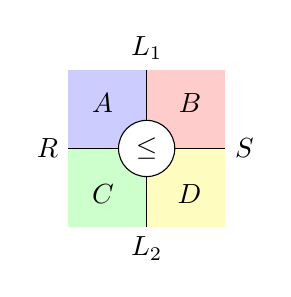
\begin{tikzpicture}[baseline]
    \path[fill=blue!20] rectangle (-1,1);
    \path[fill=red!20] rectangle (1,1);
    \path[fill=green!20] rectangle (-1,-1);
    \path[fill=yellow!25] rectangle (1,-1);
    \draw (0,0) -- (0,+1) node[anchor=south] {$L_1$};
    \draw (0,0) -- (+1,0) node[anchor=west] {$S$};
    \draw (0,0) -- (0,-1) node[anchor=north] {$L_2$};
    \draw (0,0) -- (-1,0) node[anchor=east] {$R$};
    \node[draw,circle,fill=white] (sim) {$\le$};
    \begin{scope}[inner sep=3mm]
      \node[below right] at (-1,1) {$A$};
      \node[below left] at (1,1) {$B$};
      \node[above right] at (-1,-1) {$C$};
      \node[above left] at (1,-1) {$D$};
    \end{scope}
  \end{tikzpicture}
  \quad \Rightarrow \quad
  \newcommand{\stens}{0.6}
  \begin{tikzpicture}[baseline]
    \tikzset{to path={
        .. controls ($(\tikztostart)!\stens!(\tikztostart -| \tikztotarget)$)
        and ($(\tikztotarget)!\stens!(\tikztostart -| \tikztotarget)$) ..
        (\tikztotarget) \tikztonodes}}
  
    \path (-1, +1) coordinate (R1) node[above] {$\dagger R^*$};
    \path (+1, -1) coordinate (R2) node[below] {$\dagger R_*$};
    \path (0, +1) coordinate (L1) node[above] {$ \llbracket L_1 \rrbracket^\dagger $};
    \path (0, -1) coordinate (L2) node[below] {$ \llbracket L_2 \rrbracket^\dagger $};

    
    \fill[color=red!20] (sim) to (R2) -- (+1.2,-1) -- (+1.2,0) -- cycle;
    \path[fill=red!20] rectangle (+1.2,+1);
    \fill[color=green!20] (sim) to (R1) -- (-1.2,+1) -- (-1.2,0) -- cycle;
    \path[fill=green!20] rectangle (-1.2,-1);

    \fill[color=yellow!20] (sim) to (R2) -- (L2) -- cycle;
    \fill[color=yellow!20] (0,0) to (R2) -- (L2) -- cycle;
    \fill[color=blue!20] (sim) to (R1) -- (L1) -- cycle;
    \fill[color=blue!20] (0,0) to (R1) -- (L1) -- cycle;
    
    \node[draw,circle,fill=white] (sim) {$\sqsubseteq$};
    \node[below right] at (-0.9,+1) {$\dagger \llbracket A \rrbracket$};
    \node[below left] at (+1,+1) {$\dagger \llbracket B \rrbracket$};
    \node[above right] at (-1,-1) {$\dagger \llbracket C \rrbracket$};
    \node[above left] at (0.9,-1) {$\dagger \llbracket D \rrbracket$};
    
    \draw (sim) to (R1);
    \draw (sim) -- (L1);
    \draw (sim) to (R2);
    \draw (sim) -- (L2);
  \end{tikzpicture}
\]

\subsection{Control Operators (optional, medium difficulty)}

Although we can't define things like setjmp/longjmp/context switching
directly in terms of the CompCertO semantics,
we can define them as operators on embedded games semantics
of CompCert programs,
which interpret calls to the relevant primitives
in the appropriate way.
In this part we could for example:
\begin{itemize}
  \item Give a specification of context switching in these terms
  \item Give a certified implementation at the assembly level
\end{itemize}
This would go a long way towards
a reformulation of (parts of) CCAL into RBGS.

\subsection{Processes and their Environment (optional, lesser difficulty)}

Define \emph{loaders} to ``close'' the C interface of a component.
This means we don't have to deal with memory states any more
and just get the observable behavior of a closed process.
That behavior could have a degrees of sophistication:
\begin{itemize}
  \item Just use CompCert events, but use game semantics to interpret them
  \item Still allow outgoing calls in the (semi-)closed semantics
  \item Have the loader include semantics for some standard library functions,
    and give a higher-level view of what they do
    using a new outgoing language interface.
\end{itemize}

If we do that,
we can model how closed CompCert processes interact
with the operating system,
and could give a small example like
specify and verify simple versions of
the \texttt{sort} and \texttt{uniq} commands,
then model the behavior of a
\texttt{sort|uniq}
pipeline.

Another reason to do this would be to close a gap in CompCertO,
where currently we do not prove that the initial invocation of main
(including the initial memory state)
is compatible with our calling convention.

\section{Certified Abstraction Layers}

Certified abstraction layers can be embedded into the category of effect
signatures.

The signature of a layer interface or implementation
can be encoded as an effect signature.
For example:
\begin{align*}
  E_\kw{bq} &:= \{
    \kw{enq}[v] : \mathbbm{1}, \kw{deq} : V \mid
    v \in V \} \\
  E_\kw{rb} &:= \{
    \kw{set}[i, v] \! : \! \mathbbm{1},
    \kw{get}[i] \! : \! V,
    \kw{inc}_1 \! : \! \mathbb{N},
    \kw{inc}_2 \! : \! \mathbb{N} \! \mid \!
    i \in \mathbb{N}, v \in V \}
\end{align*}

In order to handle the layer's abstract data,
we can extend signatures with state in the following way:
\[
  E@S :=
    \{ m@k : \kw{ar}(m) \times S \mid
       m \in E, k \in S \}
\]

A layer interface $L$ with a signature $E$
and states in $S$
can be interpreted as
a homomorphism $\llbracket L \rrbracket : I \multimap E@S$.
Recall that a signature homomorphism of type $I \multimap E$
chooses arguments for each possible operation.
\[
  \llbracket L \rrbracket (m@k) :=
    \bigsqcup L.m@k
\]

We introduce a special homomorphism $e^k : \dagger E@S \multimap \dagger E$
to erase the explicit abstract state and instead use
strategies as specifications, where $k \in S$
is a state.
\[
  e^k(\underline{m}ns) \mathrel{:=} \bigsqcup_{k'\in S} \underline{m@k}(n@k' \mapsto e^{k'}(s))
\]
Given an initial state $k$, the embedded specification
in terms of the game model is defined as
\[
  \llbracket L \rrbracket^k \mathrel{:=} e^k \circ \llbracket L \rrbracket^\dagger : I \multimap \dagger E
\]

Given an underlay $L$ with signature $F$ and abstract state $S_2$
a layer implementation $M$
with an overlay signature $F$
extending the abstract state to $(S_1, S_2)$
can be interpreted as
a signature homomorphism $\llbracket M \rrbracket^m :  \dagger E@S_2 \multimap F@(S_1, S_2)$
by replacing external calls to underlay primitives
in the definition of $M$ with the corresponding operations:
\[
  \llbracket M \rrbracket^m \mathrel{:=} (M.m)[e \mathrel{:=} ???]
\]
The full behavior of implementation relies on
an underlay specification $I \multimap \dagger E$.
In order to compose them together
we introduce an adapter $\iota: E \multimap E@S$
that store the state upon an invocation of an operation to the underlay
and adjoin the same state to the next
incoming move.
\[
  \iota(m@k) \mathrel{:=} \underline{m}(n \mapsto n@k)
\]
Together with the state eraser,
a layer implementation $M$
given an initial state $k=(k_1,k_2)$
can be interpret as
\[
  \llbracket M \rrbracket^k \mathrel{:=}
  e^k \circ \llbracket M \rrbracket^\dagger \circ \dagger \iota : \dagger E \multimap \dagger F
\]
Consequently, running the implementation on top of
a underlay specification $L$ yield the composition
\[
  \llbracket M \rrbracket^{k_1,k_2} \circ \llbracket L \rrbracket^{k_2} : I \multimap \dagger F
\]
The layer judgment $L_1 \vdash_R M : L_2$,
which means that a layer implementation $M$
correctly implements $L_2$ on top of  $L_1$ through
a simulation relation $R \subseteq S_2 \times S_1$,
can then be interpreted as:
\[
  L_1 \vdash_R M : L_2 \Leftrightarrow
  \forall k_2\ R\ k_1\,.\, 
\llbracket L_2 \rrbracket^{k_2} \sqsubseteq
\llbracket M \rrbracket^{k_1} \circ \llbracket L \rrbracket^{\iota_2(k_1)}
\]
where $\iota_2$ is the projection to extract underlay state from $k_1$.

\section{Related Work}

\section{Conclusion}

\bibliographystyle{ACM-Reference-Format}
\bibliography{references}

\newpage

\noindent
For now,
the rest of this document contains my previous CompCertOX write-up.

\begin{figure}[h] % fig:ex {{{
  \begin{center}
    \begin{tikzcd}[row sep=1cm, column sep=1.5cm]
      1 \ar[d, double, dash] \ar[rrr, ->>, "L''"] &&&
      \mathcal{C}@K''
        \ar[d, <->, "S"]
        \ar[r, ->>, "\llbracket C \rrbracket@K''"] &
      \mathcal{C}@K''
        \ar[ddd, <->, "R \circ S"]
      \\
      1 \ar[d, double, dash] \ar[rr, ->>, "L'"] &&
      \mathcal{C}@K'
        \ar[d, <->, "R"]
        \ar[r, ->>, "\llbracket N \rrbracket@K'"] &
      \mathcal{C}@K'
        \ar[d, <->, "R"]
      \\
      1 \ar[d, double, dash] \ar[r, ->>, "L"] &
      \mathcal{C}@K
        \ar[d, double, dash] 
        \ar[r, ->>, "\llbracket M \rrbracket@K"] &
      \mathcal{C}@K
        \ar[r, ->>, "\llbracket N \rrbracket@K"] &
      \mathcal{C}@K
        \ar[d, double, dash]
      \\
      1 \ar[d, double, dash] \ar[r, ->>, "L"] &
      \mathcal{C}@K
        \ar[d, double, dash] 
        \ar[rr, ->>, "\llbracket M + N \rrbracket@K"] &&
      \mathcal{C}@K
        \ar[r, ->>, "\llbracket C \rrbracket@K"] &
      \mathcal{C}@K
        \ar[d, double, dash] 
      \\
      1 \ar[r, ->>, "L"] &
      \mathcal{C}@K
        \ar[rrr, ->>, "\llbracket C + M + N \rrbracket@K"] &&&
      \mathcal{C}@K
    \end{tikzcd}
  \end{center}
  \caption}}

\section{Overview} %{{{

Our usual
\href{https://certikos.github.io/rbgs-papers/thesis/thesis.pdf\#chapter.4}%
  {theory of abstraction layers}
can be formulated in CompCertO's double category of
language interfaces, simulation conventions and transition systems:
\begin{itemize}
  \item A layer interface $L$ with abstract states in $K$
    is represented as $L : 1 \twoheadrightarrow \mathcal{C}@K$
  \item Clight semantics define
    $\llbracket M \rrbracket : \mathcal{C} \twoheadrightarrow \mathcal{C}$
    and lift to
    $\llbracket M \rrbracket @ K :
     \mathcal{C}@K \twoheadrightarrow \mathcal{C}@K$
  \item Abstraction relations define simulation conventions
    $R : \mathcal{C}@K' \Leftrightarrow \mathcal{C}@K$
  \item Layer correctness
    $L \vdash_R M : L'$
    is encoded as
    $L' \le_{\mathsf{id} \twoheadrightarrow R}
     \llbracket M \rrbracket @K \circ L$
\end{itemize}
\autoref{fig:ex}
demonstrates how these ingredients may fit together
in a typical situation.

The following operators
are used to formulate vertical and horizontal composition
of abstraction layers.
In the homogenous case
$(A \twoheadrightarrow A) \times
 (A \twoheadrightarrow A) \rightarrow
 (A \twoheadrightarrow A)$,
they under-approximate $\oplus$
and can therefore be implemented by linking.
\begin{itemize}
  \item Categorical composition \hfill
    $\circ :
      (B \twoheadrightarrow C) \times
      (A \twoheadrightarrow B) \rightarrow
      (A \twoheadrightarrow C) \qquad$
  \item Flat composition \hfill
    $\uplus :
      (A \twoheadrightarrow B) \times
      (A \twoheadrightarrow B) \rightarrow
      (A \twoheadrightarrow B) \qquad$
\end{itemize}
To reconnect formally with Yu's work,
we can investigate the following further:
\begin{itemize}
  \item A CompCertO transition system $L : A \twoheadrightarrow B$
    can be embedded into $\dagger A \multimap B$.
  \item The cliques of $\dagger \mathcal{C}$
    are universal abstract states.
  \item We can map between effect signatures $E$
    and the language interfaces $\mathcal{C}, \mathcal{A}$.
\end{itemize}
We can then define
a principled embedding
into game semantics or coherence spaces.

\paragraph{Status}

This draft should mostly be accurate,
however we will have to work out some of the details and kinks.
Here is a list of issues:
\begin{itemize}
  \item Components which make outgoing calls
    to functions in their own domain
    cause problems in the relationship between
    $\circ$, $\uplus$ and $\oplus$.
  \item In fact the word ``domain'' is somewhat confusing,
    more precisely it's a set of symbols
    that are reserved by the component.
\end{itemize}

%A certified abstraction layer
%$L_2 \vdash_R M : L_1$
%establishes that:
%\[
%  L_1 \le_{\mathsf{id} \twoheadrightarrow R}
%  \llbracket M \rrbracket @K_2 \circ L_2
%\]
%Various properties of the operators involved
%ensure that
%for any context $C$,
%\[
%  \llbracket C \rrbracket@K_1 \circ L_1
%  \: \le_{\mathsf{id} \twoheadrightarrow R} \:
%  \llbracket C \rrbracket@K_2 \circ \llbracket M \rrbracket@K_2 \circ L_2
%  \: \le_{\mathsf{id} \twoheadrightarrow \mathsf{id}} \:
%  \llbracket C + M \rrbracket@K_2 \circ L_2
%  \,.
%\]
%In particular,
%this enables vertical composition:
%\[
%  L_1
%  \: \le_{\mathsf{id} \twoheadrightarrow R} \:
%  \llbracket M \rrbracket@K_2 \circ L_2
%  \: \le_{\mathsf{id} \twoheadrightarrow S} \:
%  \llbracket M + N \rrbracket@K_3 \circ L_3
%\]
%On the other hand,
%the flat composition operator:
%\[
%  L_1, L_2 : A \twoheadrightarrow B
%  \vdash
%  L_1 \uplus L_2 : A \twoheadrightarrow B
%\]
%allows us to carry out a similar

%}}}

\section{Categorical structure of CompCertO semantics} %{{{

The semantic model used in CompCertO
can be organized into a double category:
\begin{itemize}
  \item the objects are language interfaces;
  \item the horizontal morphisms are open transition systems;
  \item the vertical morphisms are simulation conventions;
  \item the 2-cells are simulations.
\end{itemize}
The CompCertO paper defines
the vertical composition of simulation conventions,
but focuses on a symmetric form of horizontal composition,
meant to model linking:
\[
  {\oplus} :
    (A \twoheadrightarrow A) \times
    (A \twoheadrightarrow A) \rightarrow
    (A \twoheadrightarrow A)
\]

In this section,
I complement the constructions on CompCertO's open semantics
to make their double category structure explicit.
In particular,
I introduce the simpler and more fundamental
horizontal composition operators:
\[
  \begin{array}{c@{\:}l}
  {\circ} &:
    (B \twoheadrightarrow C) \times
    (A \twoheadrightarrow B) \rightarrow
    (A \twoheadrightarrow C)
  \\
  {\uplus} &:
    (A \twoheadrightarrow B) \times
    (A \twoheadrightarrow B) \rightarrow
    (A \twoheadrightarrow B)
  \end{array}
\]
The linking operator $\oplus$
can then be recovered or characterized as the fixed point
\[
  L_1 \oplus L_2 :=
    \mu X \cdot (L_1 \uplus L_2) \circ X
  \,.
\]

\subsection{Horizontal category} %{{{

\subsubsection{Identity} %{{{

The identity transition system $\mathsf{id}_A : A \twoheadrightarrow A$
can be defined as:
\[
  \mathsf{id}_A :=
    \langle A^\circ + A^\bullet,\: \varnothing,\: \varnothing,\: I,\: X,\: Y,\: F \rangle
\]
The components are defined by the rules:
\[
  \begin{prooftree}
    \infer0{q \mathrel{I} \iota_1(q)}
  \end{prooftree}
  \qquad
  \begin{prooftree}
    \infer0{\iota_1(q) \mathrel{X} q}
  \end{prooftree}
  \qquad
  \begin{prooftree}
    \infer0{r \mathrel{Y^{\iota_1(q)}} \iota_2(r)}
  \end{prooftree}
  \qquad
  \begin{prooftree}
    \infer0{\iota_2(r) \mathrel{F} r}
  \end{prooftree}
\]

%}}}

\subsubsection{Composition} %{{{

Suppose we have the transition systems:
\begin{align*}
  L_1 &= \langle S_1, {\rightarrow_1}, D_1, I_1, X_1, Y_1, F_1 \rangle
    : B \twoheadrightarrow C
  \\
  L_2 &= \langle S_2, {\rightarrow_2}, D_2, I_2, X_2, Y_2, F_2 \rangle
    : A \twoheadrightarrow B
\end{align*}
The composite transition system is defined as
\[
  L_1 \circ L_2 :=
  \langle S, {\rightarrow}, D_1 \cup D_2, I, X, Y, F \rangle
\]
with the following components.
States are of the form:
\[
    S := S_1 + (S_2 \times S_1)
\]
Initially, the environment question activates $L_1$:
\[
  \begin{prooftree}
    \hypo{q_C \mathrel{I_1} s_1}
    \infer1{q_C \mathrel{I} \iota_1(s_1)}
  \end{prooftree}
  \qquad
  \begin{prooftree}
    \hypo{s_1 \rightarrow_1 s_1'}
    \infer1{\iota_1(s_1) \rightarrow \iota_1(s_1')}
  \end{prooftree}
  \qquad
  \begin{prooftree}
    \hypo{s_1 \mathrel{F_1} r_C}
    \infer1{\iota_1(s_1) \mathrel{F} r_C}
  \end{prooftree}
\]
When an external call is encountered,
the question is used to activate $L_2$:
\[
  \begin{prooftree}
    \hypo{s_1 \mathrel{X_1} q_B}
    \hypo{q_B \mathrel{I_2} s_2}
    \infer2{\iota_1(s_1) \rightarrow \iota_2(s_2, s_1)}
  \end{prooftree}
\]
Execution proceeds according to $L_2$,
\[
  \begin{prooftree}
    \hypo{s_2 \rightarrow_2 s_2'}
    \infer1{\iota_2(s_2, s_1) \rightarrow \iota_2(s_2', s_1)}
  \end{prooftree}
  \qquad
  \begin{prooftree}
    \hypo{s_2 \mathrel{X_2} q_A}
    \infer1{\iota_2(s_2, s_1) \mathrel{X} q_A}
  \end{prooftree}
  \qquad
  \begin{prooftree}
    \hypo{r_A \mathrel{Y_2^{s_2}} s_2'}
    \infer1{r_A \mathrel{Y^{\iota_2(s_2, s_1)}} \iota_2(s_2', s_1)}
  \end{prooftree}
\]
until a final state of $L_2$ is reached,
at which point $L_1$ is resumed:
\[
  \begin{prooftree}
    \hypo{s_2 \mathrel{F_2} r_B}
    \hypo{r_B \mathrel{Y_1^{s_1}} s_1'}
    \infer2{\iota_2(s_2, s_1) \rightarrow \iota_1(s_1')}
  \end{prooftree}
\]

%}}}

\subsubsection{Properties} %{{{

I will write:
\begin{itemize}
  \item $L_1 \le L_2$
    to mean $L_1 \le_{\mathsf{id} \twoheadrightarrow \mathsf{id}} L_2$,
  \item $L_1 \equiv L_2$
    to mean $L_1 \le L_2 \wedge L_2 \le L_1$.
\end{itemize}
The expected properties of the horizontal
identity and categorical composition
can then be formulated in the following way.

\begin{theorem}
For a transition system $L : A \twoheadrightarrow B$,
the following property holds:
\[
    L \circ \mathsf{id}_A \equiv \mathsf{id}_B \circ L \equiv L
    \,.
\]
Moreover, for the transition systems
\[
  \begin{tikzcd}
    A \ar[r, ->>, "L_3"] &
    B \ar[r, ->>, "L_2"] &
    C \ar[r, ->>, "L_1"] &
    D \,,
  \end{tikzcd}
\]
the following property holds:
\[
    (L_1 \circ L_2) \circ L_3 \equiv L_1 \circ (L_2 \circ L_3)
\]
\begin{proof}
It should be straightforward to verify
that the identity acts as a unit for composition.
Associativity can be verified using
the simulation relation:
\[
  \begin{array}{rr}
    \hline
    L_1 \circ (L_2 \circ L_3) & (L_1 \circ L_2) \circ L_3 \\
    \hline
    \iota_1(s_1) & \iota_1(\iota_1(s_1)) \\
    \iota_2(\iota_1(s_2), s_1) & \iota_1(\iota_2(s_2, s_1)) \\
    \iota_2(\iota_2(s_3, s_2), s_1) & \iota_2(s_3, \iota_2(s_2, s_1)) \\
    \hline
  \end{array}
\]
\end{proof}
\end{theorem}

%}}}

\begin{remark}[Domains and categorical composition]
  Unlike the horizontal composition operator $\oplus$
  and the flat composition operator $\uplus$ introduced in the next section,
  categorical composition does not make use of the component's domains
  to compute the behavior of the composite transition system.
  This means that in general,
  a component may exhibit meaningful behaviors on queries outside its domain.
  This is the case in particular for $\mathsf{id}_A$,
  where the domain is $\varnothing$ but
  every possible query is associated with a behavior.
  In turn it suggests a modification to CompCertO's
  language semantics which would make them act as ``passthough''
  on queries outside of a module's domain.

  I should also note that categorical composition as
  given in this section will require modifying
  the definition of CompCertO's transition systems slightly.
  As it stands,
  a component's domain $D$ is a set of queries of
  the incoming language interface.
  However,
  for the domain $D_1 \cup D_2$ used in $L_1 \circ L_2$
  to make sense when $B \neq C$,
  we will have to change it to a language-independent
  notion of domain, for example a set of identifiers.
  Language interfaces
  would then provide a way to recognize whether queries
  are part of a domain expressed in this general way.
\end{remark}

%}}}

\subsection{Simulations} %{{{

Horizontal composition is compatible with simulations in the following sense.
Given
$L_1 : B \twoheadrightarrow C$ and $L_2 : A \twoheadrightarrow B$,
which are simulated respectively by
$L_1' : B' \twoheadrightarrow C'$ and $L_2' : A' \twoheadrightarrow B'$,
the following property holds:
\[
  \begin{prooftree}
    \hypo{L_1 \le_{S \twoheadrightarrow T} L_1'}
    \hypo{L_2 \le_{R \twoheadrightarrow S} L_2'}
    \infer2{L_1 \circ L_2 \le_{R \twoheadrightarrow T} L_1' \circ L_2'}
  \end{prooftree}
\]
Diagrammatically,
this allows us to paste simulations squares horizontally:
\[
  \begin{tikzcd}
    A \ar[r, ->>, "L_1"] \ar[d, <->, "R"] &
    B \ar[r, ->>, "L_2"] \ar[d, <->, "S"] &
    C \ar[d, <->, "T"] \\
    A' \ar[r, ->>, "L_1'"'] &
    B' \ar[r, ->>, "L_2'"'] &
    C'
  \end{tikzcd}
  \qquad \Longrightarrow \qquad
  \begin{tikzcd}
    A \ar[rr, ->>, "L_1 \circ L_2"] \ar[d, <->, "R"] &&
    C \ar[d, <->, "T"] \\
    A' \ar[rr, ->>, "L_1' \circ L_2'"'] &&
    C'
  \end{tikzcd}
\]

Note that the vertical composition of simulation squares
corresponds to the usual composition of simulations already given
in the CompCertO paper:
\[
  \begin{prooftree}
    \hypo{L_1 \le_{R \twoheadrightarrow S} L_2}
    \hypo{L_2 \le_{T \twoheadrightarrow U} L_3}
    \infer2{L_1 \le_{R \cdot T \twoheadrightarrow S \cdot U} L_3}
  \end{prooftree}
  \hspace{3em}
  \begin{tikzcd}
    A_1 \ar[r, ->>, "L_1"] \ar[d, <->, "R"] & B_1 \ar[d, <->, "S"] \\
    A_2 \ar[r, ->>, "L_2"] \ar[d, <->, "T"] & B_2 \ar[d, <->, "U"] \\
    A_3 \ar[r, ->>, "L_3"] & B_3
  \end{tikzcd}
  \quad
  \begin{tikzcd}[row sep=large]
    A_1 \ar[r, ->>, "L_1"] \ar[dd, <->, "R \cdot T"] & B_1 \ar[dd, <->, "S \cdot U"] \\ \\
    A_3 \ar[r, ->>, "L_3"] & B_3
  \end{tikzcd}
\]

One last observation is that the identity transition system
allows us to formulate the refinement of simulation conventions itself
as a simulation square.
There is a nice symmetry
with the refinement of transition systems:
\[
  \begin{tikzcd}[sep=tiny]
    A \ar[dd, double, dash, "\mathsf{id}_A"'] \ar[rr, ->>, "L_1"] &&
    B \ar[dd, double, dash, "\mathsf{id}_B"] \\
    & L_1 \le L_2 & \\
    A \ar[rr, ->>, "L_2"'] &&
    B
  \end{tikzcd}
  \hspace{5em}
  \begin{tikzcd}[sep=tiny]
    A \ar[dd, <->, "S"'] \ar[rr, double, dash, "\mathsf{id}_A"] &&
    A \ar[dd, <->, "R"] \\
    & R \sqsupseteq S & \\
    B \ar[rr, double, dash, "\mathsf{id}_B"'] &&
    B
  \end{tikzcd}
\]

%}}}

\subsection{Flat composition} %{{{

The categorical composition of two transition systems
chains them together,
directing any outgoing calls of the first
to incoming calls of the second.
I now introduce another kind of composition
which lays them out side-by-side.

\begin{definition}
The \emph{flat composition} of the transition systems
\begin{align*}
  L_1 &= \langle S_1, {\rightarrow_1}, D_1, I_1, X_1, Y_1, F_1 \rangle
    : A \twoheadrightarrow B
  \\
  L_2 &= \langle S_2, {\rightarrow_2}, D_2, I_2, X_2, Y_2, F_2 \rangle
    : A \twoheadrightarrow B
\end{align*}
is the transition system
$L_1 \uplus L_2 : A \twoheadrightarrow B$
defined as:
\[
  L_1 \uplus L_2 :=
    \langle
      S_1 + S_2, \:
      {\rightarrow}, \:
      D_1 \cup D_2, \:
      I, \: X, \: Y, \: F
    \rangle
\]
The components are defined by the following rules,
where $i \in \{1, 2\}$:
\[
  \begin{prooftree}
    \hypo{q \mathrel{I_i} s}
    \hypo{q \in D_i}
    \infer2{q \mathrel{I} \iota_i(s)}
  \end{prooftree}
  \quad
  \begin{prooftree}
    \hypo{s \rightarrow_i s'}
    \infer1{\iota_i(s) \rightarrow \iota_i(s')}
  \end{prooftree}
  \quad
  \begin{prooftree}
    \hypo{s \mathrel{X_i} q}
    \infer1{\iota_i(s) \mathrel{X} q}
  \end{prooftree}
  \quad
  \begin{prooftree}
    \hypo{r \mathrel{Y_i^s} s'}
    \infer1{r \mathrel{Y^{\iota_i(s)}} \iota_i(s')}
  \end{prooftree}
  \quad
  \begin{prooftree}
    \hypo{s \mathrel{F_i} r}
    \infer1{\iota_i(s) \mathrel{F} r}
  \end{prooftree}
\]
\end{definition}

\noindent
I suspect the following properties hold when applicable:
\begin{itemize}
  \item $\mathsf{id} \uplus L \equiv L \uplus \mathsf{id} \equiv L$
  \item $(L_1 \uplus L_2) \circ L \equiv (L_1 \circ L) \uplus (L_2 \circ L)$
\end{itemize}

\begin{remark}
It may be necessary for $\uplus$
to act as \emph{passthrough}
for queries outside of its domain.
This would enable the correspondence with $\oplus$
described in the next section.

The main difficulty is that
this can only be done when $A = B$,
so we would want to achieve this effect indirectly.
One option would be to expect language semantics
to be \emph{passthrough} outside their domain
and to have a nondeterministic choice between the components
when we're outside the domain of both.
That is to say,
each component is \emph{inhibited by the other's domain}
instead of \emph{enabled by its own}.
In normal situations the behavior of both components
would be the same in the ``gap'' between the domains,
so it would only be nondeterminism on a formal level.
\end{remark}

%}}}

\subsection{Linking} %{{{

The linking operator $\oplus$
can be described as the limit:
\[
  L_1 \oplus L_2 :=
  \bigvee_{n \in \mathbb{N}}
    (L_1 \uplus L_2)^n \circ \bot_{D_1 \cup D_2}
\]
where:
\begin{itemize}
  \item
    $L^n$ is the $n$-fold composition $L \circ \cdots \circ L$;
  \item
    $D_1$ and $D_2$ are the respective domains of $L_1$ and $L_2$;
  \item
    $\bot_D$ is undefined on its domain $D$ and
    \emph{passthrough} outside of it.
\end{itemize}
Note in particular that $\mathsf{id} \equiv \bot_\varnothing$.

For certified abstraction layers,
our main interest is that $\oplus$ can be used
to established a connexion between
the various kinds of transition system compositions
and the semantics of the linked program.

\begin{theorem}
For two Clight programs $M$ and $N$,
the linked program $M + N$ is a correct implementation of
$\llbracket M \rrbracket \oplus \llbracket N \rrbracket$:
\[
    \llbracket M \rrbracket \oplus \llbracket N \rrbracket \le
    \llbracket M + N \rrbracket
\]
\begin{proof}
A linking theorem for the Asm language has already been proved.
The Clight proof should be similar.
\end{proof}
\end{theorem}

Then the key fact is that $\circ$ and $\uplus$
are both under-approximations of $\oplus$;
in other words, they are both implemented by linking:
\begin{align*}
  \llbracket M \rrbracket \circ \llbracket N \rrbracket \: &\le \:
    \llbracket M \rrbracket \oplus \llbracket N \rrbracket \: \le \:
    \llbracket M + N \rrbracket \\
  \llbracket M \rrbracket \uplus \llbracket N \rrbracket \: &\le \:
    \llbracket M \rrbracket \oplus \llbracket N \rrbracket \: \le \:
    \llbracket M + N \rrbracket
\end{align*}
The first property in particular
can be visualized as the simulation square:
\begin{equation}
  \begin{tikzcd}
    \mathcal{C} \ar[r, "\llbracket N \rrbracket"] \ar[d, double, dash] &
    \mathcal{C} \ar[r, "\llbracket M \rrbracket"] &
    \mathcal{C} \ar[d, double, dash] \\
    \mathcal{C} \ar[rr, "\llbracket M + N \rrbracket"'] & &
    \mathcal{C}
  \end{tikzcd}
  \label{eqn:linkingsquare}
\end{equation}

%}}}

\subsection{String diagrams} %{{{

Like 2-categories,
double categories admit a string diagram calculus where:
\begin{itemize}
  \item objects are represented by regions,
  \item horizontal morphisms are represented by vertical lines,
  \item vertical morphisms are represented by horizontal lines,
  \item 2-cells are represented by points.
\end{itemize}

The diagrams I have drawn so far
efficiently convey the type structure of the semantic framework;
they describe
the way language interfaces,
transition systems and simulation conventions
compose and interact.
But the \emph{simulation proofs} themselves
are literally found in the \emph{gaps} between
these entities.

String diagrams are useful because they turn this hierarchy on its head,
and offer a compelling visualization of the ways
complex simulations can be assembled from simpler ones.
A basic simulation square $f \le_{R \twoheadrightarrow S} g$ is drawn as:
\[
  \begin{tikzcd}[sep=small]
    A \ar[rr, ->>, "f"] \ar[dd, <->, "R"'] &&
    B \ar[dd, <->, "S"] \\
    & \phi & \\
    C \ar[rr, ->>, "g"'] &&
    D
  \end{tikzcd}
  \qquad \qquad
  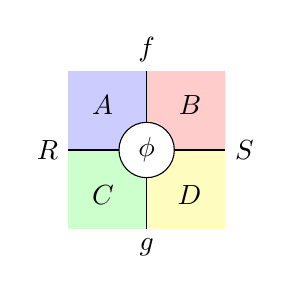
\begin{tikzpicture}[baseline]
    \path[fill=blue!20] rectangle (-1,1);
    \path[fill=red!20] rectangle (1,1);
    \path[fill=green!20] rectangle (-1,-1);
    \path[fill=yellow!25] rectangle (1,-1);
    \draw (0,0) -- (0,+1) node[anchor=south] {$f$};
    \draw (0,0) -- (+1,0) node[anchor=west] {$S$};
    \draw (0,0) -- (0,-1) node[anchor=north] {$g$};
    \draw (0,0) -- (-1,0) node[anchor=east] {$R$};
    \node[draw,circle,fill=white] (sim) {$\phi$};
    \begin{scope}[inner sep=3mm]
      \node[below right] at (-1,1) {$A$};
      \node[below left] at (1,1) {$B$};
      \node[above right] at (-1,-1) {$C$};
      \node[above left] at (1,-1) {$D$};
    \end{scope}
  \end{tikzpicture}
\]

Much information can be elided from string diagrams.
Identity transition systems and simulation conventions
can be omitted completely.
Objects can be associated with a color,
eliminating redundant labeling.
For example,
here are depictions of
a simulation convention refinement property ($R \sqsupseteq S$),
a transition system refinement property ($L_1 \le L_2$),
and of the linking property (\ref{eqn:linkingsquare}):
\[
  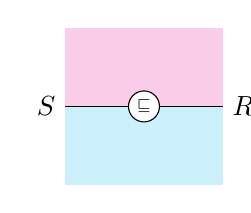
\begin{tikzpicture}[baseline]
    \path[fill=magenta!20] (-1,1) rectangle (1,0);
    \path[fill=cyan!20] (-1,0) rectangle (1,-1);
    \draw (-1,0) node[left] {$S$}
      -- (0,0) node[draw,circle,fill=white,inner sep=0.5mm] {\tiny $\sqsubseteq$}
      -- (1,0) node[right,overlay] {$R$};
  \end{tikzpicture}
  \qquad \qquad
  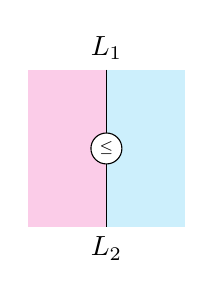
\begin{tikzpicture}[baseline]
    \path[fill=magenta!20] (-1,1) rectangle (0,-1);
    \path[fill=cyan!20] (0,1) rectangle (1,-1);
    \draw (0,1) node[above] {$L_1$}
      -- (0,0) node[draw,circle,fill=white,inner sep=0.5mm] {\tiny $\le$}
      -- (0,-1) node[below] {$L_2$};
  \end{tikzpicture}
  \qquad \qquad
  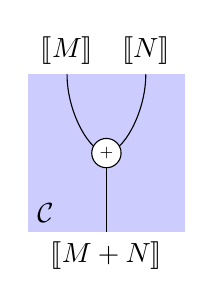
\begin{tikzpicture}[baseline]
    \path[fill=blue!20] (-1,-1) rectangle (1,1);
    \begin{scope}
      \draw (-0.5, +1) node[above] {$\llbracket M \rrbracket$}
        .. controls +(-90:0.5) and +(180:0.2) .. (0,0);
      \draw (+0.5, +1) node[above] {$\llbracket N \rrbracket$}
        .. controls +(-90:0.5) and +(0:0.2) .. (0,0);
      \draw (0,0) -- (0,-1) node[below] {$\llbracket M + N \rrbracket$};
    \end{scope}
    \node[draw,circle,fill=white,inner sep=0.5mm] {\tiny $+$};
    \node[above right] at (-1,-1) {$\mathcal{C}$};
  \end{tikzpicture}
\]

\noindent
Skipping ahead,
here is a string diagram rendition of \autoref{fig:ex}.
\[
  \pgfdeclarelayer{nodes}
  \pgfsetlayers{main,nodes}
  \newcommand{\stens}{0.6}
  \begin{tikzpicture}[baseline,yscale=1.2,xscale=1.5]
    \footnotesize
    \tikzset{to path={
      .. controls ($(\tikztostart)!\stens!(\tikztostart -| \tikztotarget)$)
              and ($(\tikztotarget)!\stens!(\tikztostart -| \tikztotarget)$) ..
      (\tikztotarget) \tikztonodes}}

    % Boundary labels
    \begin{scope}
      \path (1,4) coordinate (L2) node[above] {$L''$};
      \path (2.5,4) coordinate (C) node[above] {$\llbracket C \rrbracket$};
      \path (3.5,3) coordinate (S) node[right] {$S$};
      \path (3.5,2) coordinate (R) node[right] {$R$};
      \path (0,0) coordinate (L) node[below] {$L$};
      \path (2,0) coordinate (T) node[below] {$\llbracket M+N+C \rrbracket$};
    \end{scope}

    % Simulation proofs
    \begin{pgfonlayer}{nodes}
      % Layer correctness
      \tikzset{every node/.style={rounded corners,draw,fill=white,inner sep=1mm}}
      \path (1,3) coordinate (LC2) node {$L' \vdash_S N : L''$};
      \path (0.5,2) coordinate (LC1) node {$L \vdash_R M : L'$};
      % Linking
      \tikzset{every node/.style={circle,draw,fill=white,inner sep=0.5mm}}
      \path (1.5,1.33) coordinate (LK1) node {$+$};
      \path (2,0.66) coordinate (LK2) node {$+$};
      % Parametricity
      \tikzset{every node/.style={circle,draw,fill=black,inner sep=0.5mm}}
      %\node (P2) at (4,2) {};
      %\node (P3) at (3,2) {};
    \end{pgfonlayer}

    % Regions
    \fill[color=magenta!20] (L2) to (LC2) -- (S) |- cycle;
    \fill[color=yellow!20] (LC2) to (LC1) -- (R) |- cycle;
    \fill[color=cyan!20] (LC1) to (L) -| (R) -- cycle;

    % Transition systems
    \begin{scope}[line width=1pt,inner sep=0.2mm]
      % \draw (L2) to (LC2) to node[above left,pos=0.75] {$L'$} (LC1) to (L);
      \draw (T) to (LK2) to (LK1) to node[below left,pos=0.3] {$\llbracket M \rrbracket$} (LC1);
      \draw (LC2) to node[above right,pos=0.6] {$\llbracket N \rrbracket$} (LK1);
      \draw (LK2) to (C);
    \end{scope}

    % Simulation conventions
    \begin{scope}
      \draw (LC2) to (S);
      \draw (LC1) to (R);
    \end{scope}

    % Region labels
%    \begin{scope}[opacity=0.4]
%      \node[below right] at (-0.5,1) {$1$};
%      \node[above left] at (4,0) {$K$};
%      \node[left] at (4,3.5) {$K'$};
%      \node[below left] at (4,5) {$K''$};
%    \end{scope}
  \end{tikzpicture}
\]
Here the white region corresponds to
the empty language interface $1$,
whereas the colored regions correspond to
a version of the $\mathcal{C}$ language interface
extended to carry the various kinds of abstract states
used by the layer interfaces $L$, $L'$ and $L''$.
From the outer boundary of the diagram,
we can read the simulation property
\[
  \llbracket C \rrbracket@K'' \circ L''
  \le_{1 \twoheadrightarrow S \cdot R}
  \llbracket M + N + C \rrbracket@K \circ L
  \,.
\]
The diagram is a proof of this property,
constructed from the following components:
\begin{itemize}
  \item Layer correctness properties of the form
    \[
      L' \le_{\mathsf{id} \twoheadrightarrow R} \llbracket M \rrbracket@K \circ L
      \,,
    \]
    depicted as rectangular boxes.
  \item The linking property (\ref{eqn:linkingsquare}),
    lifted to operate with abstract state
    \[
      \llbracket M \rrbracket@K \circ \llbracket N \rrbracket@K
      \le_{\mathsf{id} \twoheadrightarrow \mathsf{id}}
      \llbracket M + N \rrbracket@K
      \,,
    \]
    depicted with a plus symbol.
  \item The compatibility of language semantics with abstraction relations
    \[
      \llbracket C \rrbracket@K'
      \le_{R \twoheadrightarrow R}
      \llbracket C \rrbracket@K
      \,,
    \]
    depicted as crossings between the horizontal lines ($R$)
    and vertical lines ($\llbracket C \rrbracket$).
\end{itemize}

%}}}

%}}}

\section{Certified abstraction layers} %{{{

I will use the notations and concepts outlined in
\href{https://certikos.github.io/rbgs-papers/thesis/thesis.pdf\#chapter.4}{Chapter 4}
of my thesis.
In particular,
\href{https://certikos.github.io/rbgs-papers/thesis/thesis.pdf#section.4.4}{\S 4.4}
reframes our CompCertX-based approach
into our more abstract formalism
and is a starting point for the following definitions.

\subsection{Abstract states} %{{{

In CompCertX,
the memory model is extended with an \emph{abstract state} component
which is used to specify the behavior of underlay primitives.

To extend CompCertO in a similar way,
given a set $K$ of abstract states,
we can introduce an operator to transform the language interface $A$
into the language interface $A@K$
where every question and answer
is annotated with an element of $K$.

\begin{definition}
For a language interface
$A = \langle A^\circ, A^\bullet \rangle$
we define the language interface:
\[
    A@K := \langle A^\circ \times K, \: A^\bullet \times K \rangle
    \,.
\]
\end{definition}

Then,
a transition system $L : A \twoheadrightarrow B$
can be lifted to $L@K : A@K \twoheadrightarrow B@K$,
which maintains an abstract state component
and threads it through the computation.

\begin{definition}
For a transition system
$L = \langle S, {\rightarrow}, D, I, X, Y, F \rangle$,
we define:
\[
    L@K \: := \:
      \langle S \times K, \: {\rightarrow} \times {=}_K, \:
            D \times K, \: I \times {=}_K, \: X \times {=}_K, \:
            Y_K, \: F \times {=}_K \rangle
\]
where the relation $Y_K$ is defined by the rule:
\[
  \begin{prooftree}
    \hypo{n \mathrel{Y^s} s'}
    \infer1{n@{k'} \mathrel{Y_K^{s@k}} s'@k'}
  \end{prooftree} 
\]
\end{definition}

Most of the relations involved in $L@K$
simply thread this component through unchanged (${-} \times {=}_K$).
At external calls,
we update the abstract state with
its value in the environment's answer.

A similar construction can be carried out for simulation conventions.

\begin{definition}
For a simulation convention $\mathbb{R} : A \leftrightarrow B$
with $\mathbb{R} = \langle W, \mathbb{R}^\circ, \mathbb{R}^\bullet \rangle$,
we define the simulation convention
$\mathbb{R}@K : A@K \leftrightarrow B@K$
in the following way:
\[
  \mathbb{R}@K \: := \:
    \langle
      W, \:
      \mathbb{R}^\circ \times {=}, \:
      \mathbb{R}^\bullet \times {=}
    \rangle
\]
\end{definition}

Together,
these definitions define a \emph{double endofunctor}
on the double category of
transition systems, simulation conventions and simulations.
The corresponding properties
are given as follows.

\begin{theorem}
  For the transition systems
  $L_1 : A \twoheadrightarrow B$ and
  $L_2 : B \twoheadrightarrow C$,
  we have:
  \[
    \mathsf{id}_A@K \equiv \mathsf{id}_{A@K}
    \qquad
    (g \circ f)@K \equiv g@K \circ f@K
  \]
  For the simulation conventions
  $R : A \leftrightarrow B$ and $S : B \leftrightarrow C$,
  we have:
  \[
    \epsilon_A@K \equiv \epsilon_{A@K}
    \qquad
    (R \cdot S)@K \equiv R@K \cdot S@K
  \]
  Finally,
  extending with abstract state preserves simulation squares:
  \[
    \begin{tikzcd}[row sep=large,column sep=large]
      A_1 \ar[r, ->>, "L_1"] \ar[d, <->, "R_A"'] &
      B_1 \ar[d, <->, "R_B"] \\
      A_2 \ar[r, ->>, "L_2"'] & B_2
    \end{tikzcd}
    \quad \Longrightarrow \quad
    \begin{tikzcd}[row sep=large, column sep=large]
      A_1@K \ar[r, ->>, "L_1@K"] \ar[d, <->, "R_A@K"'] &
      B_1@K \ar[d, <->, "R_B@K"] \\
      A_2@K \ar[r, ->>, "L_2@K"'] & B_2@K
    \end{tikzcd}
  \]
\end{theorem}

These properties essentially mean that
entire simulation diagrams
can be extended with abstract states at once.
For example,
if the following simulations hold:
\[
  \begin{tikzcd}[sep=large]
    A \ar[r, ->>, "f"] \ar[d, <->, "R"] &
    B \ar[r, ->>, "g"] &
    C \ar[r, ->>, "h"] \ar[d, <->, "S"] &
    D \ar[dd, <->, "T"]
    \\
    E \ar[rr, ->>, "x"] \ar[d, <->, "U"] &&
    F \ar[d, <->, "V"] &
    \\
    X \ar[rr, ->>, "\phi"] &&
    Y \ar[r, ->>, "\psi"] &
    Z
  \end{tikzcd}
\]
then we can conclude that the following simulations hold as well:
\[
  \begin{tikzcd}[row sep=large]
    A@K \ar[r, ->>, "f@K"] \ar[d, <->, "R@K"] &
    B@K \ar[r, ->>, "g@K"] &
    C@K \ar[r, ->>, "h@K"] \ar[d, <->, "S@K"] &
    D@K \ar[dd, <->, "T@K"]
    \\
    E@K \ar[rr, ->>, "x@K"] \ar[d, <->, "U@K"] &&
    F@K \ar[d, <->, "V@K"] &
    \\
    X@K \ar[rr, ->>, "\phi@K"] &&
    Y@K \ar[r, ->>, "\psi@K"] &
    Z@K
  \end{tikzcd}
\]
This will be especially useful for lifting
properties established in CompCertO
to the context of certified abstraction layers,
allowing for example versions of the
compiler correctness or linking properties
extended to include abstract state:
\[
  \begin{tikzcd}[row sep=large, column sep=huge]
    \mathcal{C}@K
      \ar[r, ->>, "\llbracket M \rrbracket@K"]
      \ar[d, <->, "\mathbb{C}@K"'] &
    \mathcal{C}@K
      \ar[d, <->, "\mathbb{C}@K"] \\
    \mathcal{A}@K
      \ar[r, ->>, "\llbracket C(M) \rrbracket@K"'] &
    \mathcal{A}@K
  \end{tikzcd}
  \qquad
  \begin{tikzcd}[sep=large]
    \mathcal{C}@K
      \ar[r, ->>, "\llbracket M \rrbracket@K"]
      \ar[d, double, dash] &
    \mathcal{C}@K
      \ar[r, ->>, "\llbracket N \rrbracket@K"] &
    \mathcal{C}@K
      \ar[d, double, dash] \\
    \mathcal{C}@K
      \ar[rr, ->>, "\llbracket M + N \rrbracket@K"'] &&
    \mathcal{C}@K
  \end{tikzcd}
\]


%}}}

\subsection{Layer interfaces} %{{{

Per the definitions in my thesis and our LICS'20 paper,
a layer interface can be described as a family of specifications:
\[
    \sigma^m : K \rightarrow \mathcal{P}^1(N \times K)
\]
where $(m \mathbin: N) \in E$ is an operation of the layer's signature.
In the case of the $\mathcal{C}$ language interface of CompCertO,
operations are of the form:
\[
    f(\vec{v}) : \mathsf{val}
    \qquad
    \text{where}
    \qquad
    f \in \mathsf{val}
    \qquad
    \vec{v} \in \mathsf{val}^*
\]

A layer interface specified in this style
can easily be represented as a CompCertO transition system
$\hat{\sigma} : 1 \twoheadrightarrow \mathcal{C}@K$,
defined as:
\[
  \hat{\sigma} := \langle
    \mathsf{val} \times \mathsf{mem} \times K,
    \varnothing,
    D,
    I,
    \varnothing,
    \varnothing,
    F
  \rangle
\]
A call into this transition system involves a single state.
At invocation,
we immediately query $\sigma$ to obtain the call's outcome
and save it in the transition system's state:
\[
  \begin{prooftree}
    \hypo{\sigma^{f(\vec{v})}(k) \ni (v', k')}
    \infer1{f(\vec{v})@m@k \mathrel{I} (v', m, k')}
  \end{prooftree}
\]
This single state admits no transition but is immediately final:
\[
  \begin{prooftree}
    \infer0{(v', m, k') \mathrel{F} v'@m@k'}
  \end{prooftree}
\]

The domain $D$ has to be specified in addition to $\sigma$,
which does not carry this information.
Alternatively,
we could use a more sophisticated embedding,
where $\sigma$ is defined in terms of a more abstract
effect signature $E$,
and where we specify a correspondance between
the operations of $E$ and $\mathcal{C}$ calls.

Using the definitions above,
the semantics of a Clight program $M$
on top of a layer interface
$L : 1 \twoheadrightarrow \mathcal{C}@K$
can be given as
\[
  \llbracket M \rrbracket @K \circ L \: : \:
  1 \twoheadrightarrow \mathcal{C}@K
  \,.
\]

%}}}

\subsection{Abstraction relations} %{{{

In CompCertX-based CertiKOS,
the abstraction relation between
an overlay with abstract states in $K_1$ and
an underlay with abstract states in $K_2$
is given as a pair of relations:
\[
  R^\mathsf{r} \subseteq K_1 \times K_2
  \qquad
  R^\mathsf{m} \subseteq K_1 \times \mathsf{mem}
\]
We also associate with each layer a set of global variables $G$
such that:
\[
  \begin{prooftree}
    \hypo{k_1 \mathrel{R^\mathsf{r}} m_2}
    \hypo{m_2 \cong_G m_2'}
    \infer2{k_1 \mathrel{R^\mathsf{r}} m_2'}
  \end{prooftree}
\]
where $\cong_G$ denotes the usual $\mathsf{Mem.unchanged\_on}$
relationship asserting that the two memories
associate the same contents to the global variables in $G$.

In CompCertO,
we can use these relations to define a
memory-extension-based simulation convention
$R : \mathcal{C}@K_1 \Leftrightarrow \mathcal{C}@K_2$
which captures CertiKOS-style abstraction between
overlay and underlay behaviors:
\begin{gather*}
 {\begin{prooftree}
    \hypo{k_1 \mathrel{R^\mathsf{r}} k_2}
    \hypo{k_1 \mathrel{R^\mathsf{m}} m_2}
    \hypo{m_1 \le_\mathsf{m} m_2}
    \hypo{m_1 \mathrel\text{no-perms-on} G}
    \hypo{\vec{v}_1 \le_\mathsf{v} \vec{v}_2}
    \infer5{f(\vec{v}_1)@m_1@k_1 \mathrel{R^\circ} f(\vec{v}_2)@m_2@k_2}
  \end{prooftree}}
\\[1em]
 {\begin{prooftree}
    \hypo{k_1 \mathrel{R^\mathsf{r}} k_2}
    \hypo{k_1 \mathrel{R^\mathsf{m}} m_2}
    \hypo{m_1 \le_\mathsf{m} m_2}
    \hypo{m_1 \mathrel\text{no-perms-on} G}
    \hypo{v'_1 \le_\mathsf{v} v'_2}
    \infer5{v'_1@m_1@k_1 \mathrel{R^\bullet} v'_2@m_2@k_2}
  \end{prooftree}}
\end{gather*}
Then we can
formulate the layer correctness property
$L \vdash_R M : L'$ as
\[
    L' \le_{\mathsf{id} \twoheadrightarrow R}
    \mathsf{Clight}(M)@K \circ L
    \,.
\]

%}}}

%}}}

\section{Coherence spaces} %{{{

%}}}

\section{Effect signatures} %{{{

%}}}

\end{document}
 %%% Local Variables: 
 %%% mode: LaTeX
 %%% TeX-command-extra-options: "-shell-escape"
 %%% End:
